\apendice{Documentación de usuario}

\section{Introducción}
Este apéndice tiene como objetivo brindar a los usuarios los pasos necesarios para instalar y utilizar \textit{PlanLMS}. Se incluye a continuación información detallada sobre los requisitos mínimos para ejecutar la aplicación, pasos que el usuario debe seguir para instalar la aplicación en su dispositivo y una guía de uso.

\section{Requisitos de usuarios}
En esta sección se describen los requisitos mínimos que debe de cumplir el dispositivo del usuario para poder ejecutar correctamente \textit{PlanLMS}.

\subsection{Requisitos del Sistema} 
\begin{itemize}
    \item \textbf{Versión mínima Android:} 5.0 (API 21, \textit{Lollipop})
    \item \textbf{Versión objetivo Android:} 14.0 (API 34, \textit{Upside Down Cake})
\end{itemize}

\subsection{Requisitos Hardware}
La aplicación requiere de un dispositivo con acceso a Internet para la obtención de los datos del usuario de Moodle, así como la gestión de tareas personales, es decir, la comunicación con la base de datos.

\section{Instalación}
Actualmente la aplicación dispone de los archivos de instalación para dispositivos Android, estos se encuentran en la sección \textit{Releases} en el repositorio de GitHub.

\begin{enumerate}
    \item Acceder al siguiente repositorio de GitHub: \url{https://github.com/jpg1011/TFG-GestorTareasMoodle}.
    \item Acceder a la sección de \textit{Releases}, que se encuentra en la parte derecha.
    \item Localizar la versión más reciente y acceder a \textit{Assets}.
    \item Descargar el archivo con extensión \texttt{.apk}.
    \item Una vez descargado el archivo en el dispositivo, abrir el archivo para proceder con la instalación.

    Es necesario tener activada la opción \textit{Permitir aplicaciones de fuentes desconocidas}.
    \item Seguir la instrucciones del dispositivo para finalizar la instalación.
\end{enumerate}

\section{Manual del usuario}
A continuación, se describen todas las acciones que puede realizar un usuario de PlanLMS. Se detallarán todas las funcionalidades, así como todos los pasos a seguir para poder usar de forma eficiente cada una de las funcionalidades.

\subsection{Inicio de sesión}
\begin{figure}[H]
    \centering
    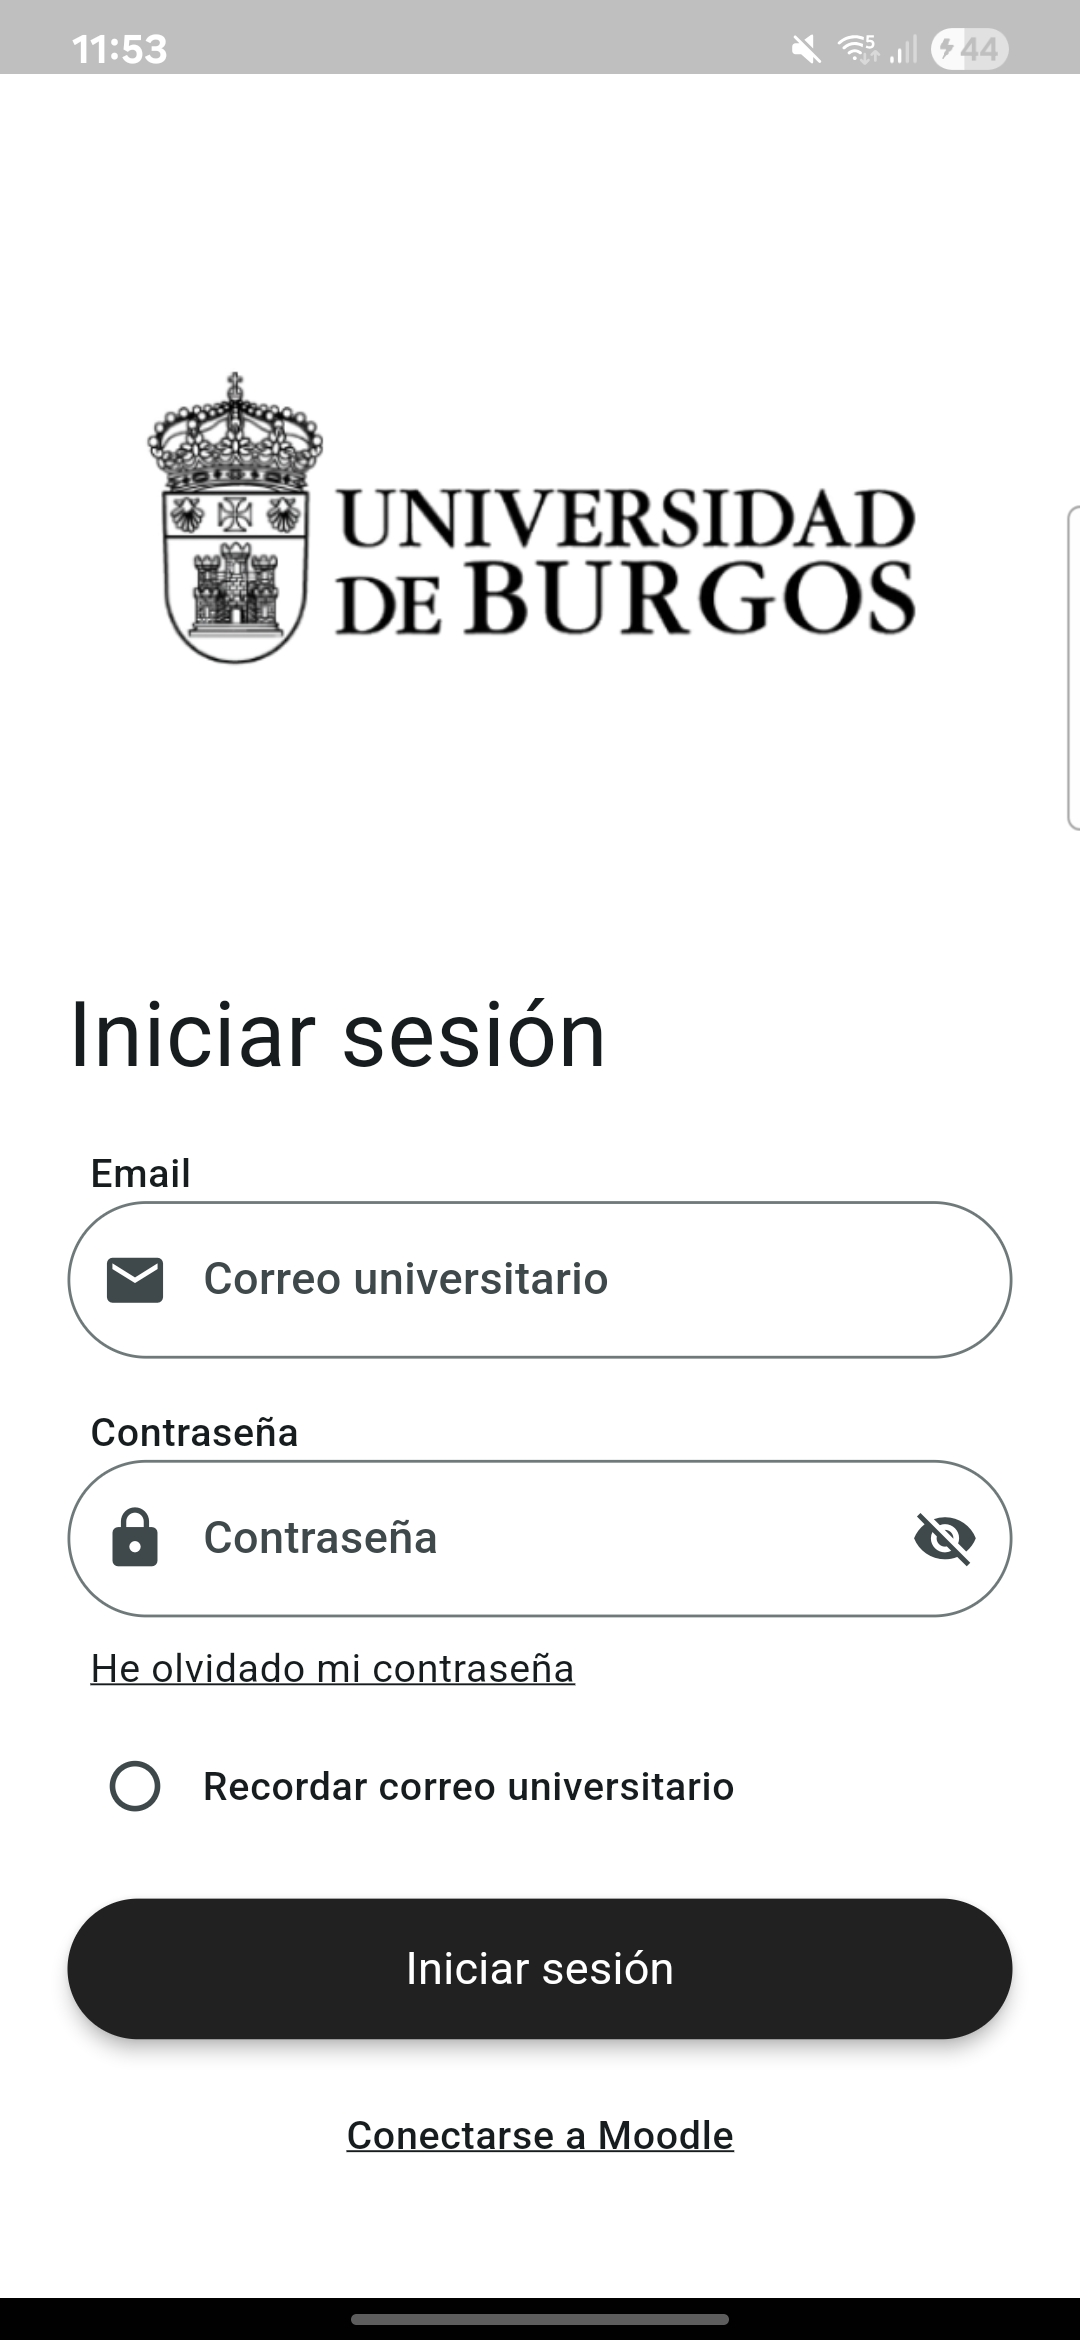
\includegraphics[width=0.4\linewidth]{img/inicio_sesion.jpg}
    \caption{Inicio de sesión de PlanLMS}
    \label{fig:inicio_sesion}
\end{figure}

En la figura \ref{fig:inicio_sesion} aparece el inicio de sesión que se compone de dos campos para introducir las credenciales de Moodle del usuario. Debajo hay un texto que redirige a la página de recuperaciónde contraseñas, en caso de no recordar la contraseña. Un \textit{checkbutton} que permite recordar el correo del usuario y el botón de acceso a la aplicación.

Por otra parte, esta el texto \textit{Conectarse a Moodle}. Al presionar dicho texto, se mostrará un pequeño diálogo, en el que se podrá introducir la \textit{URL} del servidor a conectar. Además, se incluye un sistema que verifica si la \textit{URL} introducida se trata de una plataforma Moodle.
\begin{figure}[H]
  \centering
  \begin{floatrow}
    \ffigbox
      {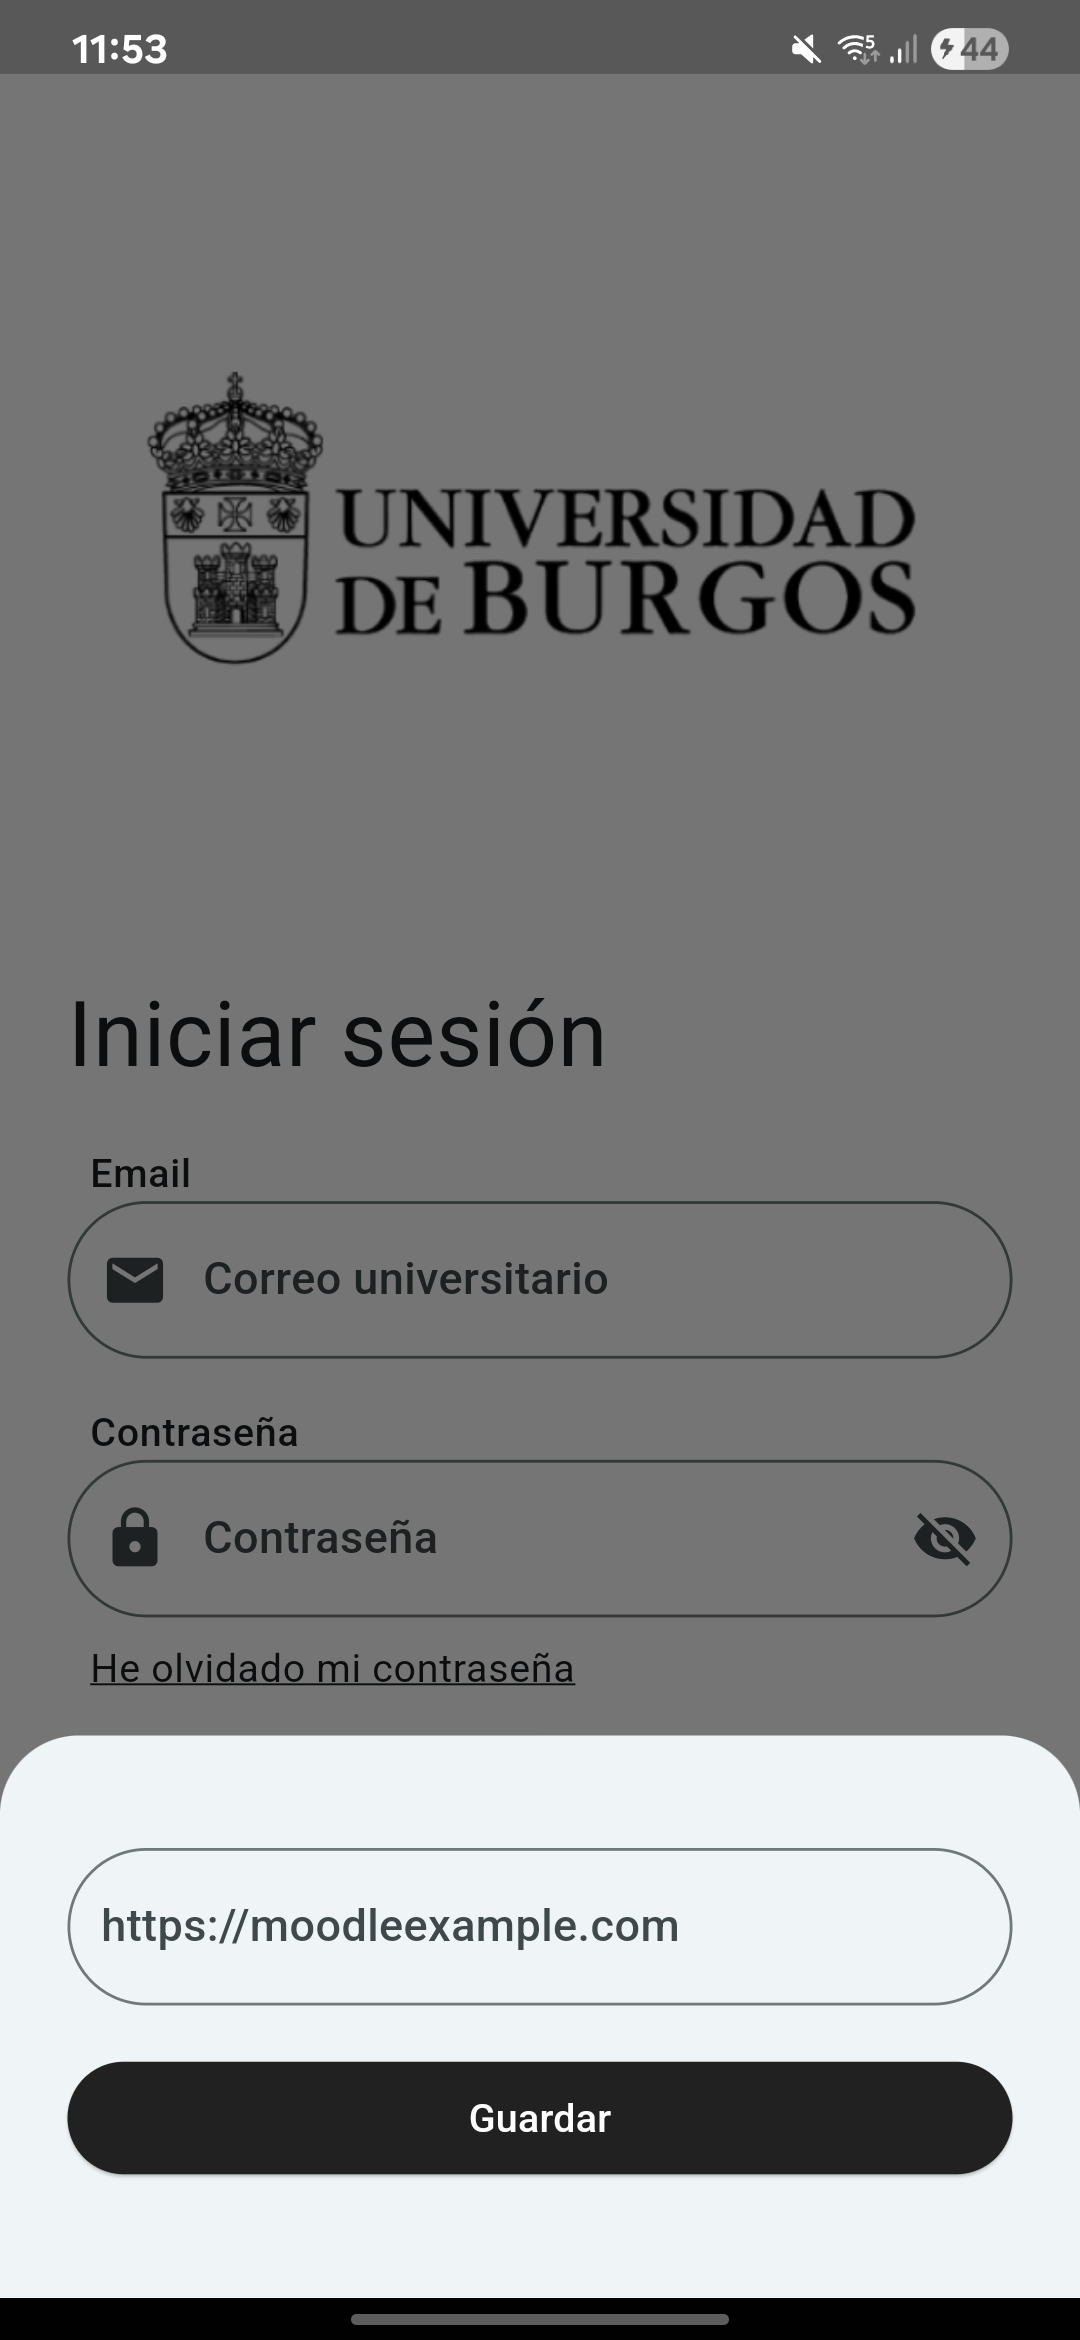
\includegraphics[width=0.5\linewidth]{img/conexion_moodle.jpg}}
      {\caption{Diálogo para conectarse a un Moodle}\label{fig:conexion_moodle}}
    \hfill
    \ffigbox
      {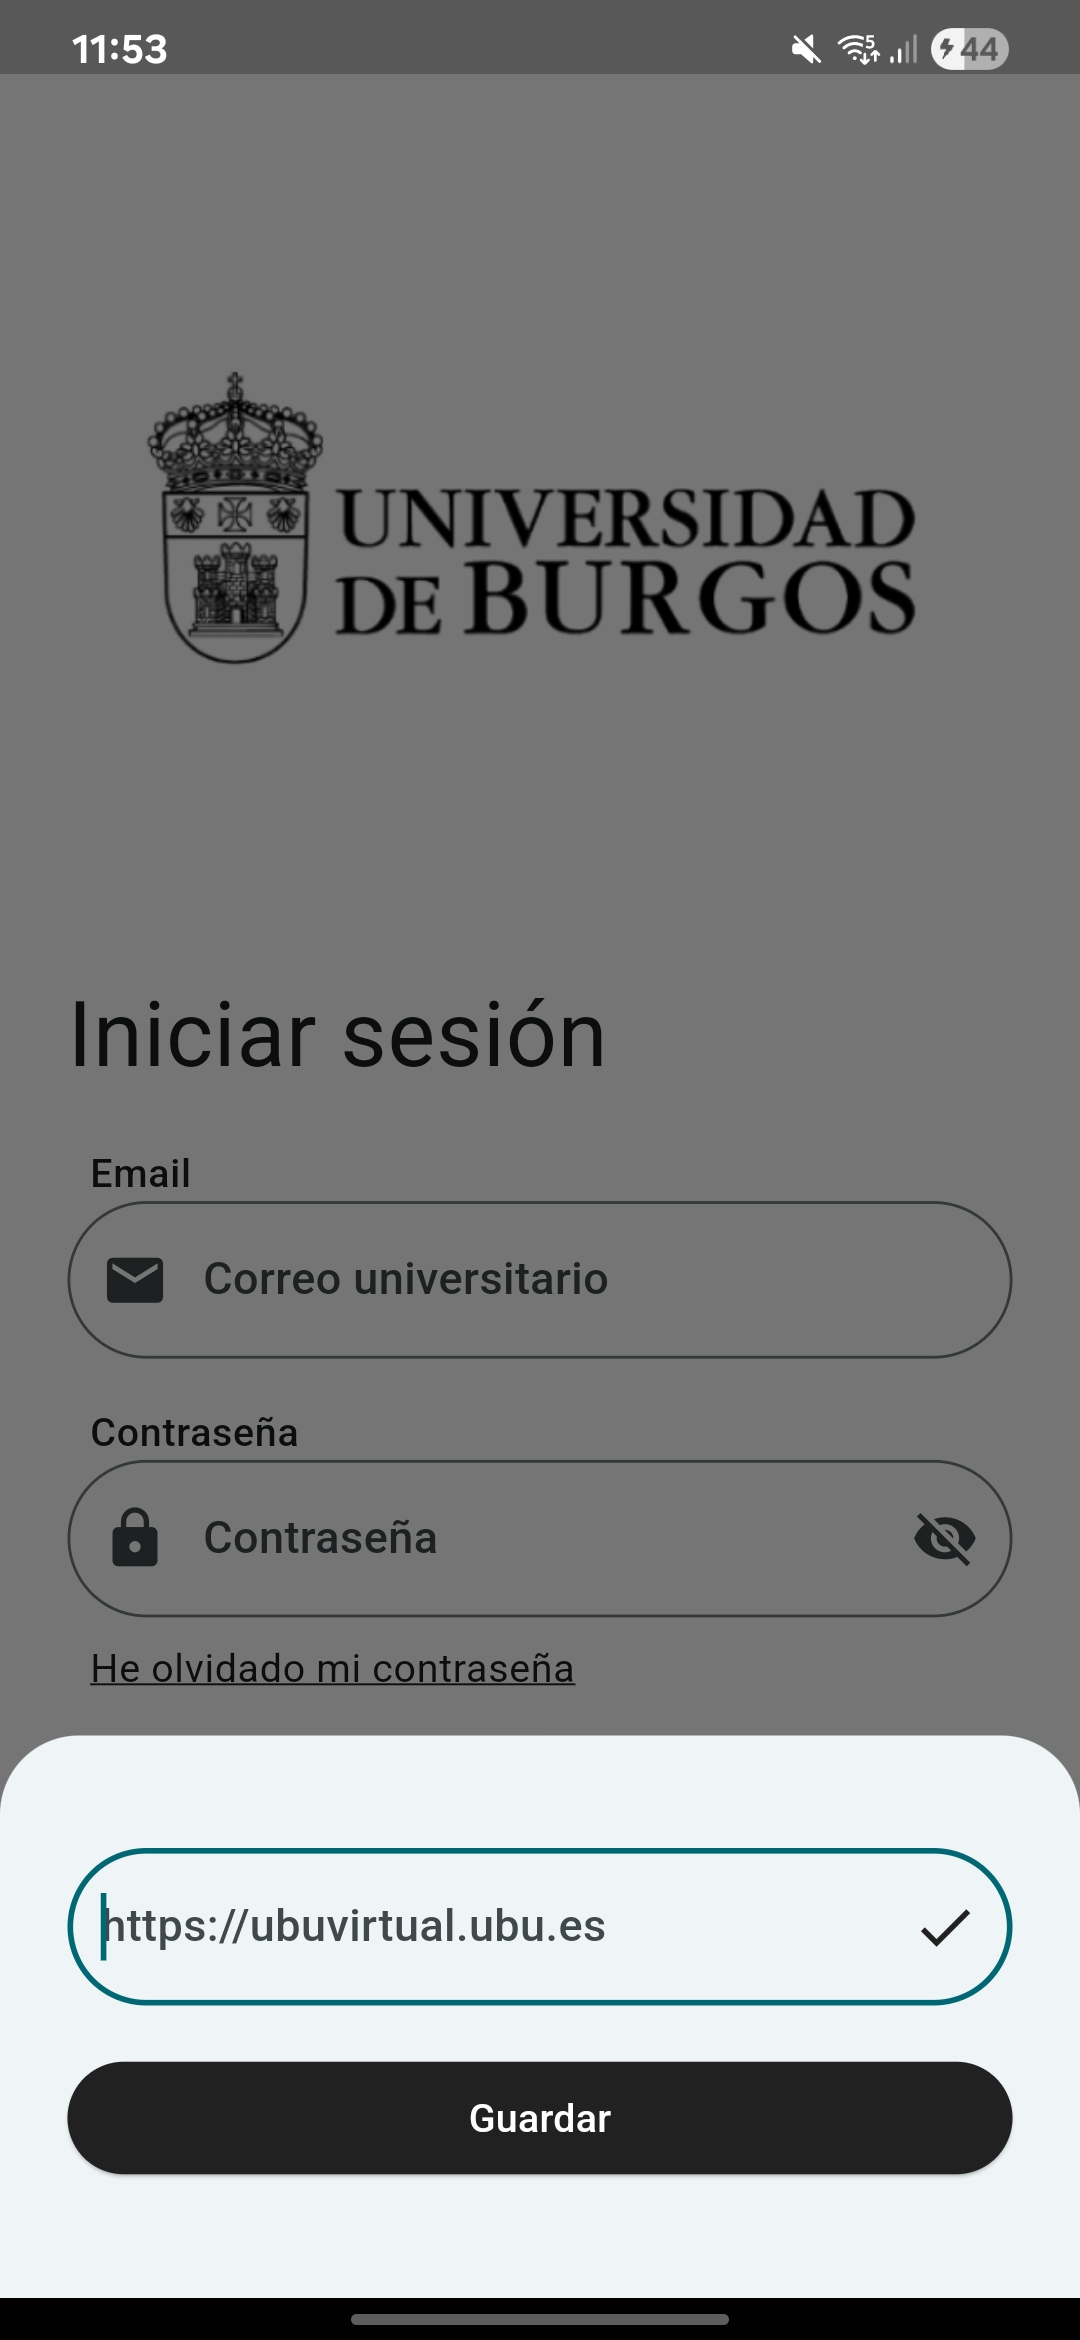
\includegraphics[width=0.5\linewidth]{img/conexion_ejemplo.jpg}}
      {\caption{Ejemplo de conexión}\label{fig:conexion_ejemplo}}
  \end{floatrow}
\end{figure}

Al presionar el botón \textit{Iniciar sesión}, se empezarán a obtener los siguientes datos de Moodle del usuario:
\begin{itemize}
    \item Información del usuario
    \item Cursos del usuario
    \item Tareas y cuestionarios de los cursos del usuario
   \item Entregas y calificaciones de las tareas y cuestionarios 
\end{itemize}
La duración del proceso de inicio de sesión puede variar en función de la cantidad de información que se vaya a extraer.

\subsection{Pantalla principal}
La primera pantalla que el usuario visualizará tras iniciar sesión, será la pantalla principal donde el usuario tendrá acceso a la siguientes funcionalidades de \textit{PlanLMS}:
\begin{itemize}
    \item Diagrama de Gantt
    \item Tareas personales
    \item Sistema de filtrado
\end{itemize}

Además, en la parte superior derecha hay un botón que se trata del cierre de sesión.
\begin{figure}[H]
    \centering
    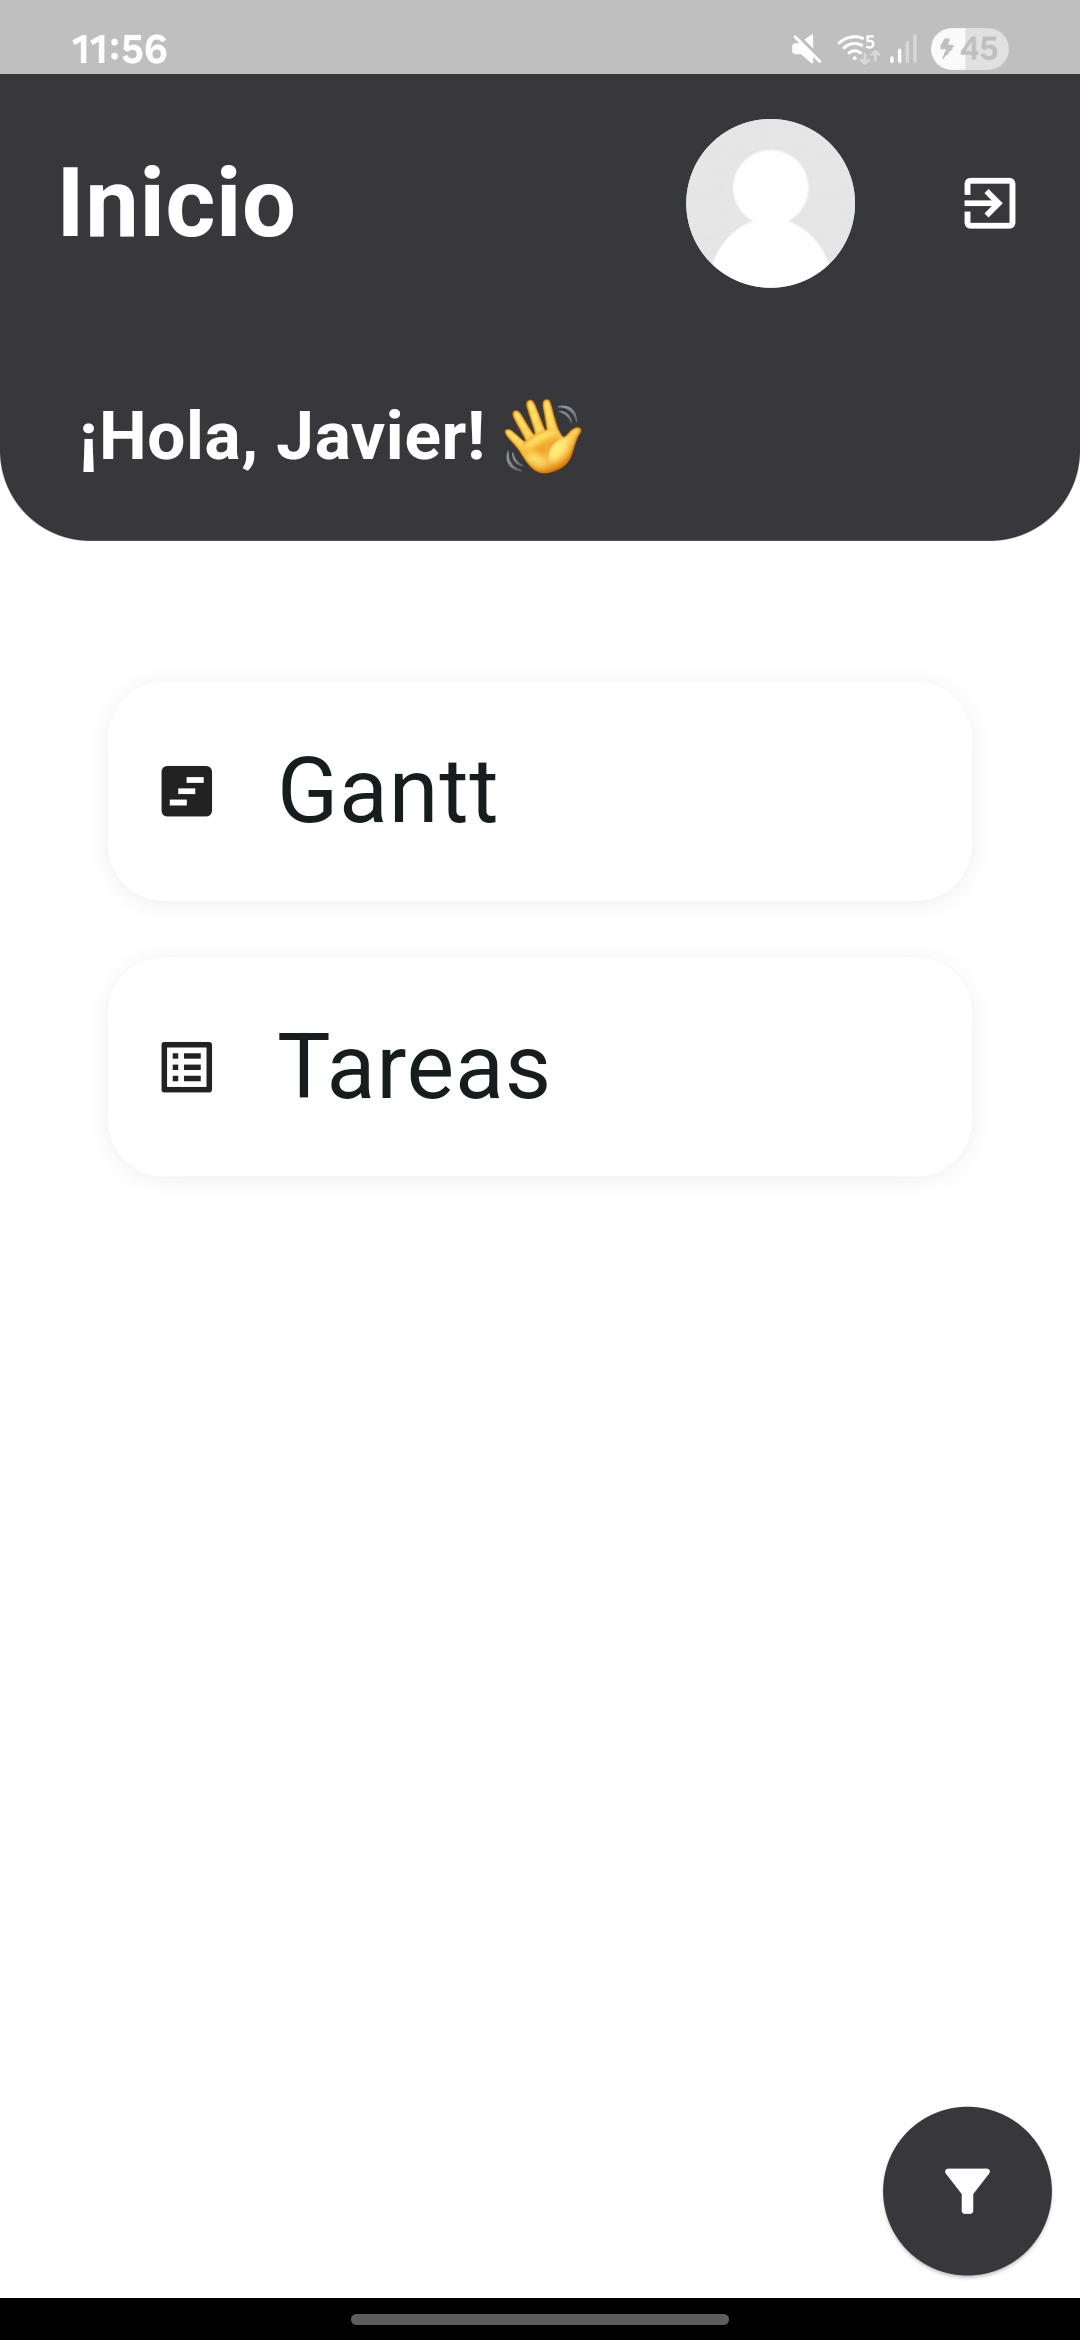
\includegraphics[width=0.4\linewidth]{img/pantalla_principal.jpg}
    \caption{Pantalla principal de PlanLMS}
    \label{fig:pantalla_principal}
\end{figure}

\subsection{Sistema de filtrado}
Para acceder a esta función basta con pulsar el botón situado en la esquina inferior derecha de la figura \ref{fig:pantalla_principal}. Al ser pulsado, aparecerá un diálogo en medio de la pantalla con todos los filtros disponibles. Algunos filtros solo afectan a algunas funcionalidades de la aplicación:
\begin{itemize}
    \item \textbf{Filtrado de cursos:} Diagrama de Gantt y Tareas Personales.
    \item \textbf{Filtrado de actividades:} Diagrama de Gantt.
    \item \textbf{Filtrado por fechas:} Diagrama de Gantt y Tareas Personales.
    \item \textbf{Filtrado por fechas disponibles:} Diagrama de Gantt.
\end{itemize}

\begin{figure}[H]
  \centering
  \begin{floatrow}
    \ffigbox
      {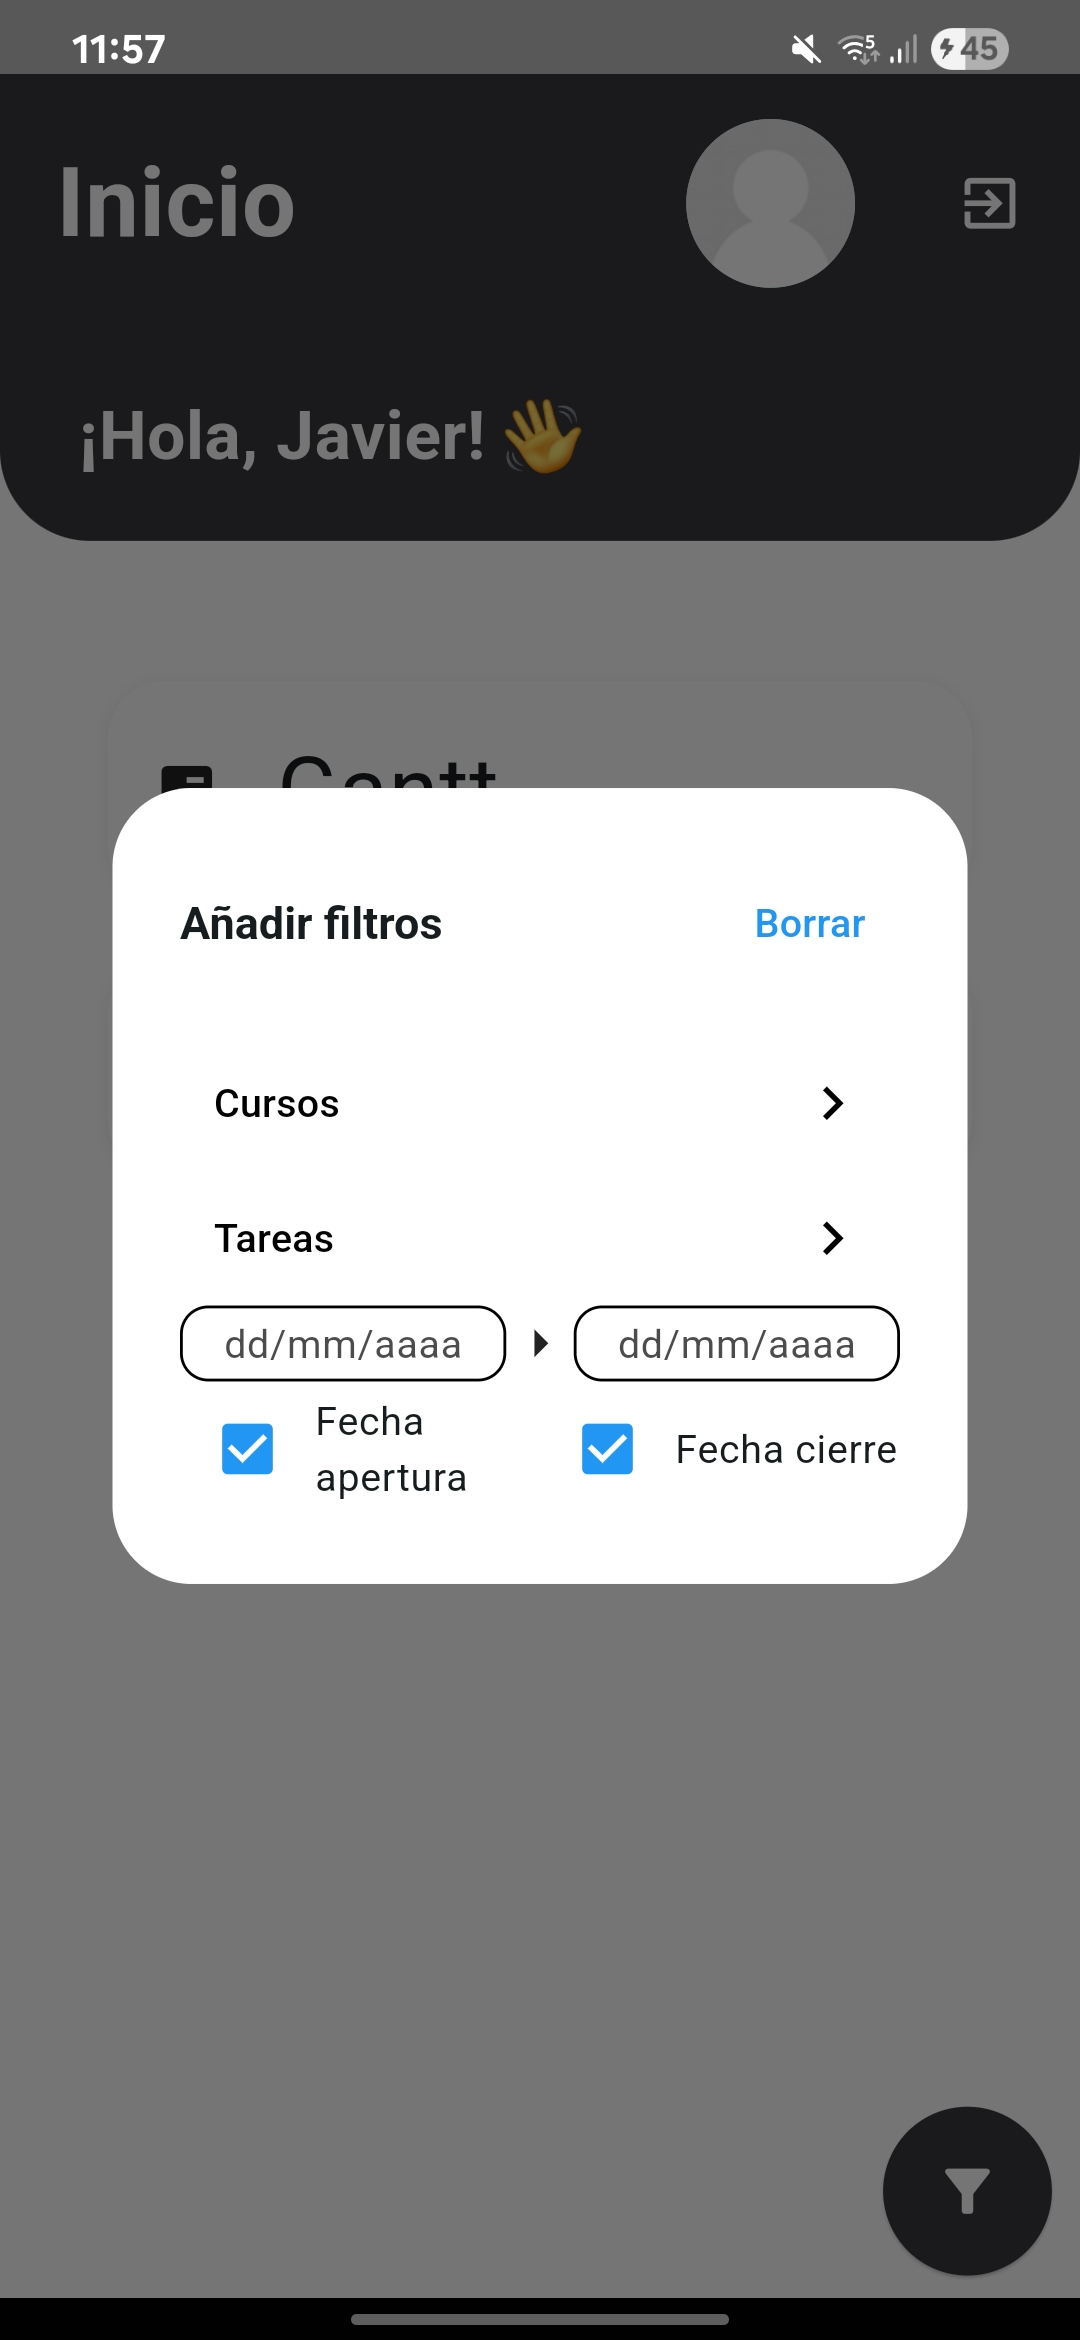
\includegraphics[width=0.5\linewidth]{img/filtros.jpg}}
      {\caption{Diálogo de filtros}\label{fig:filtros}}
    \hfill
    \ffigbox
      {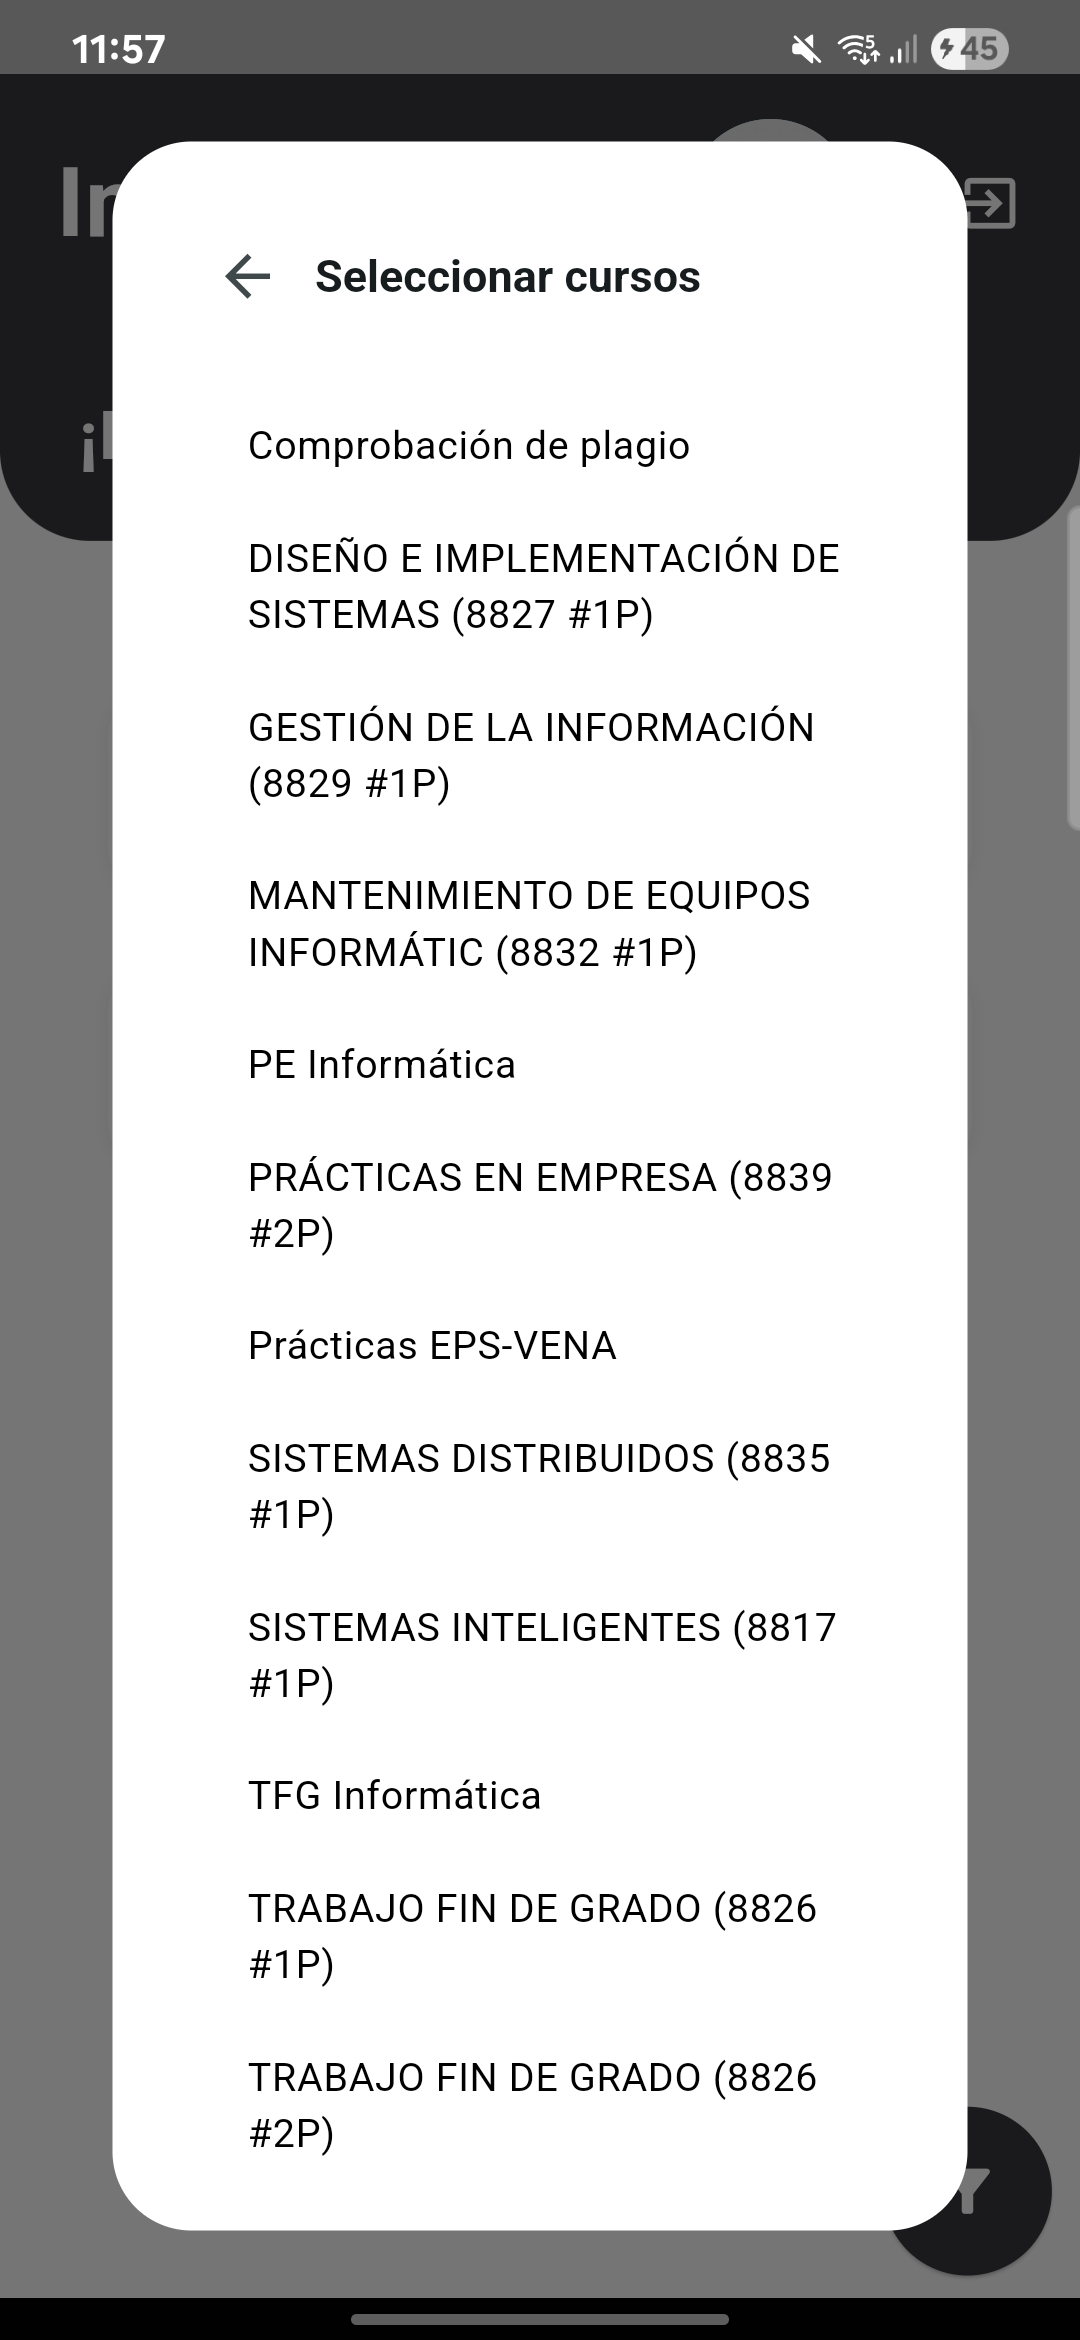
\includegraphics[width=0.5\linewidth]{img/filtros_cursos.jpg}}
      {\caption{Filtrado de cursos}\label{fig:filtros_cursos}}
  \end{floatrow}
\end{figure}
     
\begin{figure}[H]
    \centering
    {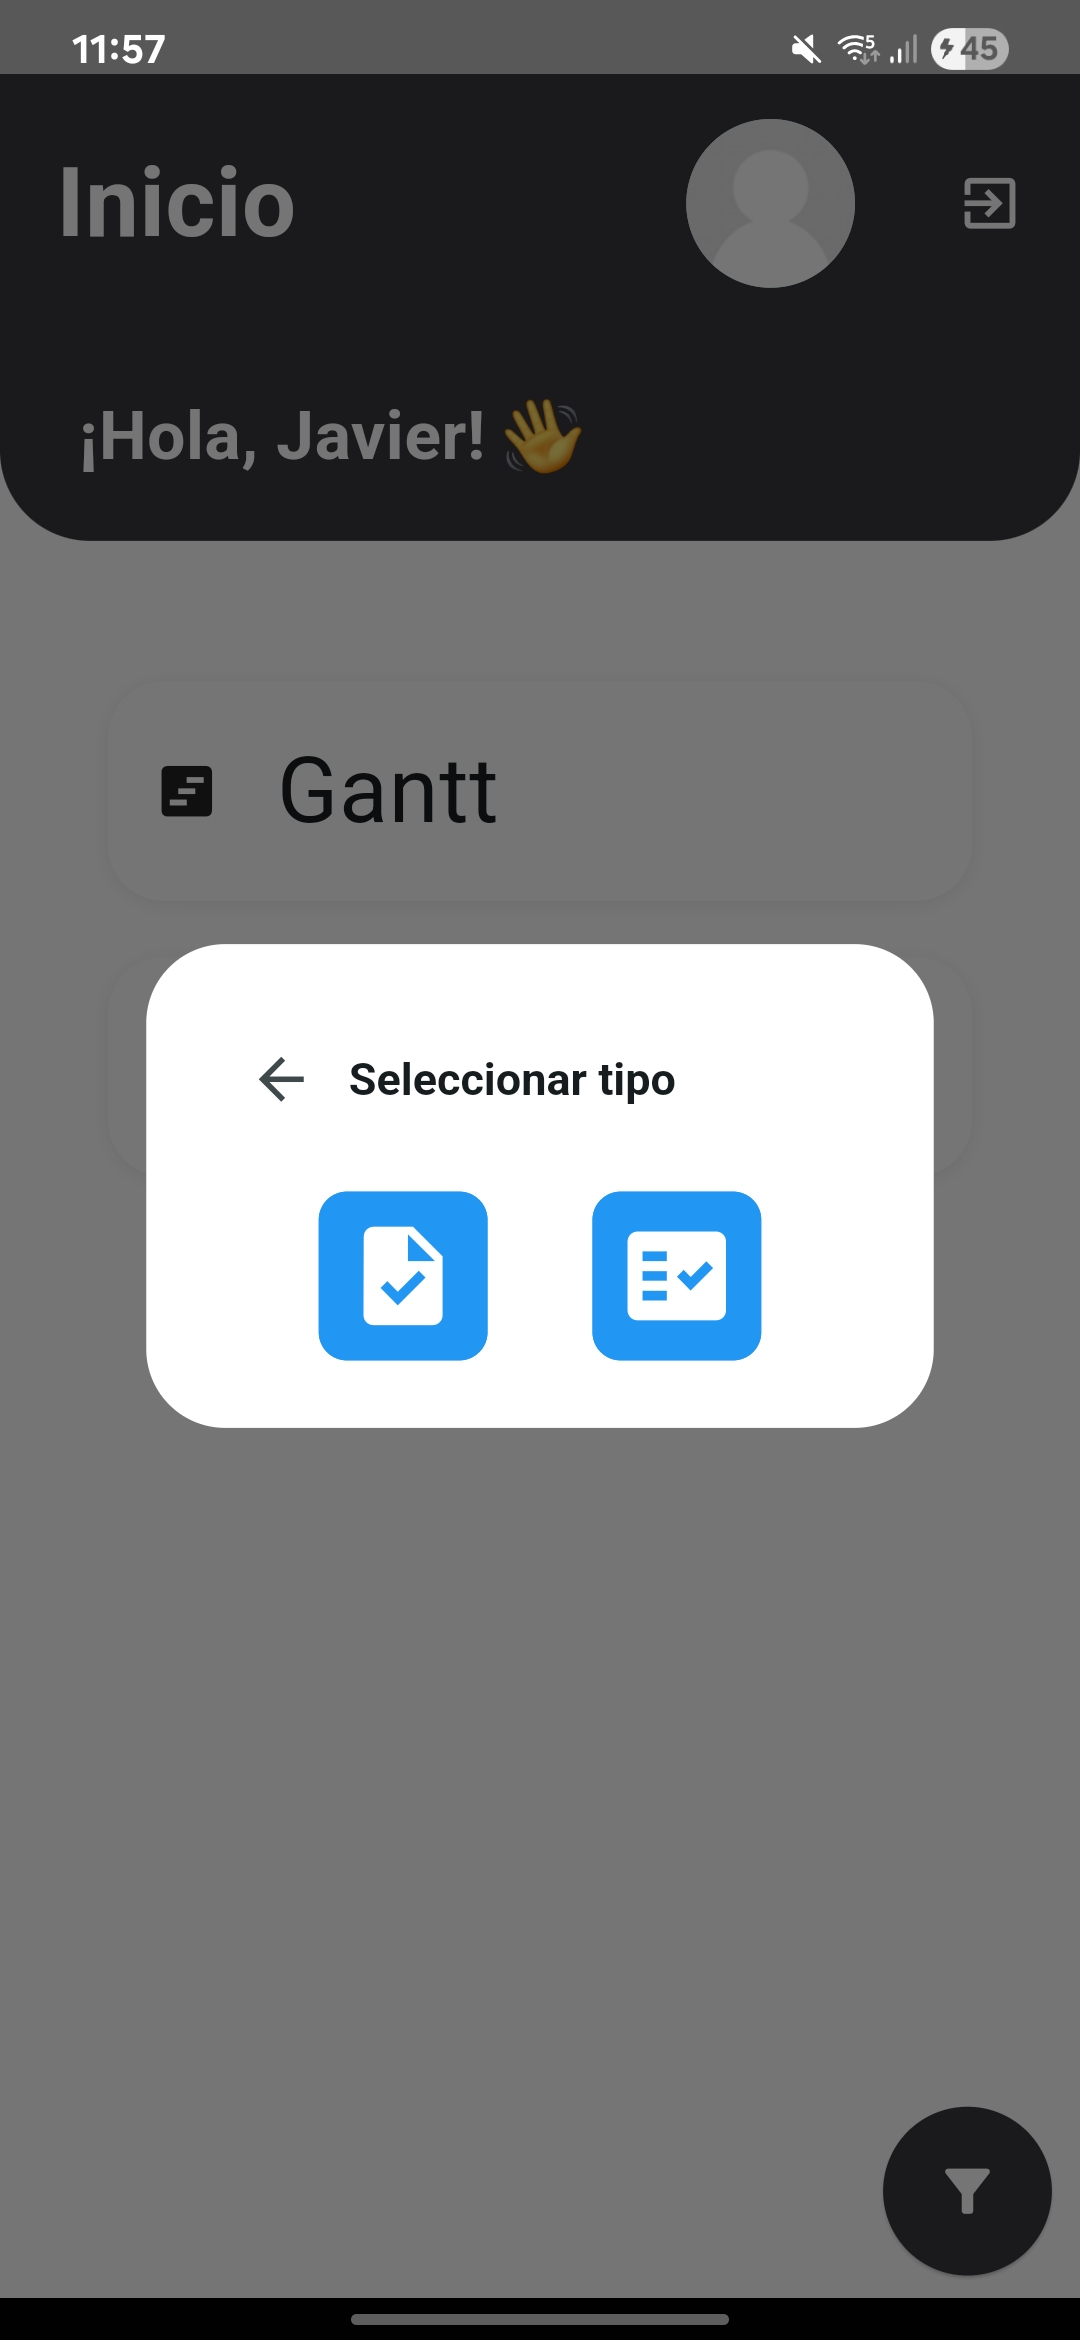
\includegraphics[width=0.25\linewidth]{img/filtros_actividades.jpg}}
     {\caption{Filtrado de actividades}
     \label{fig:filtros_actividades}}
\end{figure}

\subsubsection{Funcionamiento de los filtros}
A continuación se detalla el funcionamiento de cada uno de los filtros y como estos afectan a la aplicación.

\textbf{Filtrado de cursos}

Al acceder al diálogo \ref{fig:filtros_cursos}, se muestra una lista con todos los cursos del usuario. Por defecto, se filtrarían todos los cursos (aunque aparezcan como deseleccionados). Si se pulsa en el nombre de cada curso, este se marcaría y se filtrarían solo aquellos cursos que estén seleccionados.

\textbf{Filtrado de actividades}

Al acceder al diálogo \ref{fig:filtros_actividades}, se muestran dos iconos que por defecto se encuentran activados, por lo tanto, se filtrarían ambos tipos de actividades. En el caso de querer descartar alguna, basta con desmarcar la opción.

\textbf{Filtrado de fechas}

En el diálogo de filtros \ref{fig:filtros}, el tercer filtro disponible permite filtrar las fechas de tres formas diferentes:
\begin{itemize}
    \item Actividades a partir de una fecha
    \item Actividades anteriores a una fecha
    \item Actividades entre dos fechas
\end{itemize}


\textbf{Filtrado de fechas disponibles}

El último filtro permite filtrar aquellas actividades que por configuración carecen de fecha de apertura o de cierre, o incluso ambas. Consiste en dos casillas que en función de si están marcadas o no, mostrarán actividades con la disponibilidad de esas fechas.

\subsubsection{Diagrama de Gantt}
Una de las pantallas a las que se puede acceder desde la \textit{Pantalla Principal} \ref{fig:pantalla_principal} es el diagrama de Gantt. Esta pantalla permite al usuario visualizar las actividades filtradas en un diagrama de Gantt, que además puede ser personalizado con filtros para modificar su apariencia.
\begin{figure}[H]
  \centering
  \begin{floatrow}
    \ffigbox
      {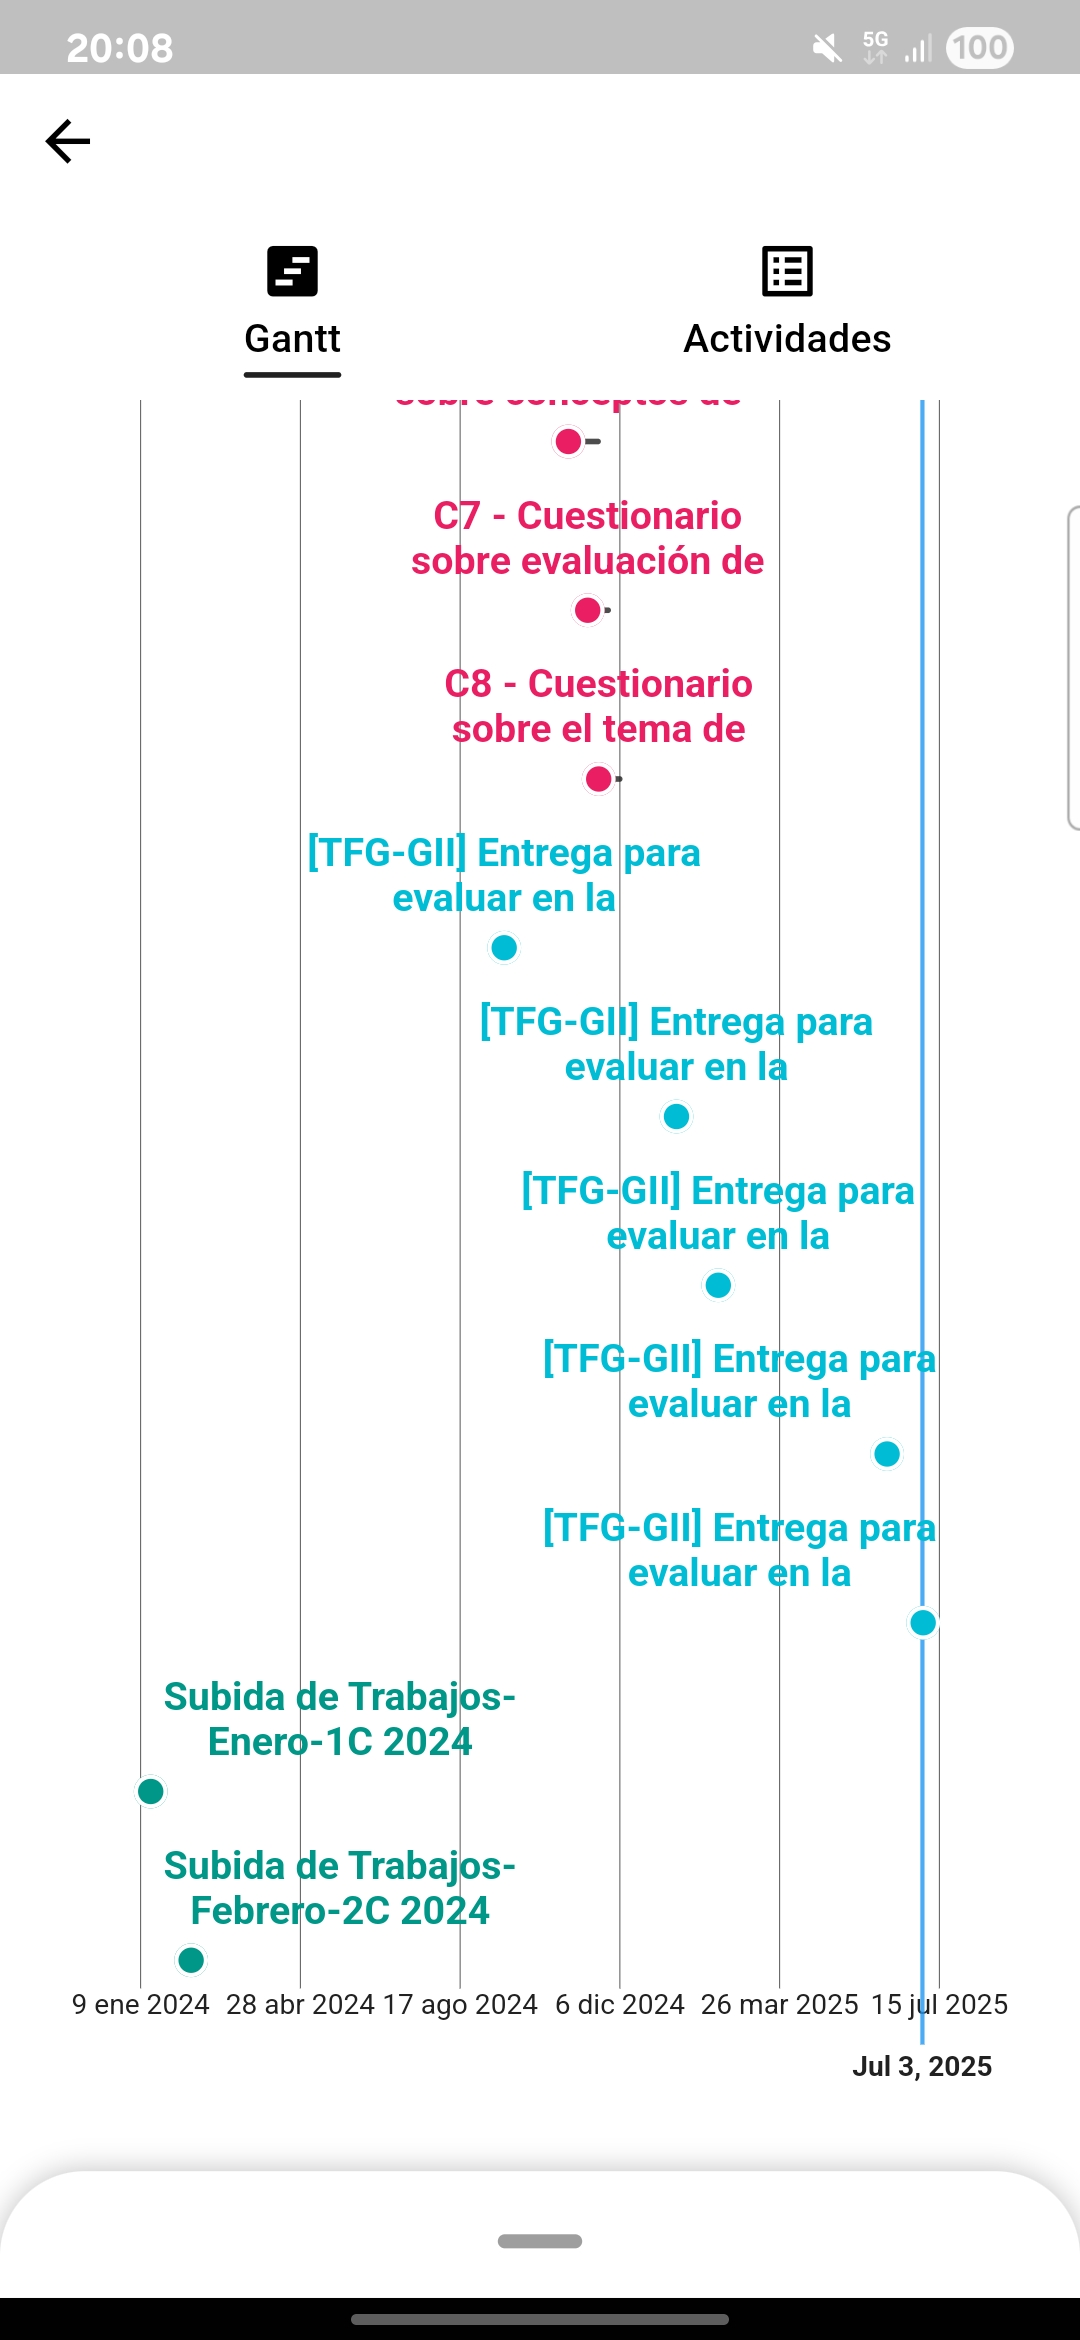
\includegraphics[width=0.5\linewidth]{img/diagrama_gantt.jpg}}
      {\caption{Pantalla de diagrama de Gantt}\label{fig:diagrama_gantt}}
    \hfill
    \ffigbox
     {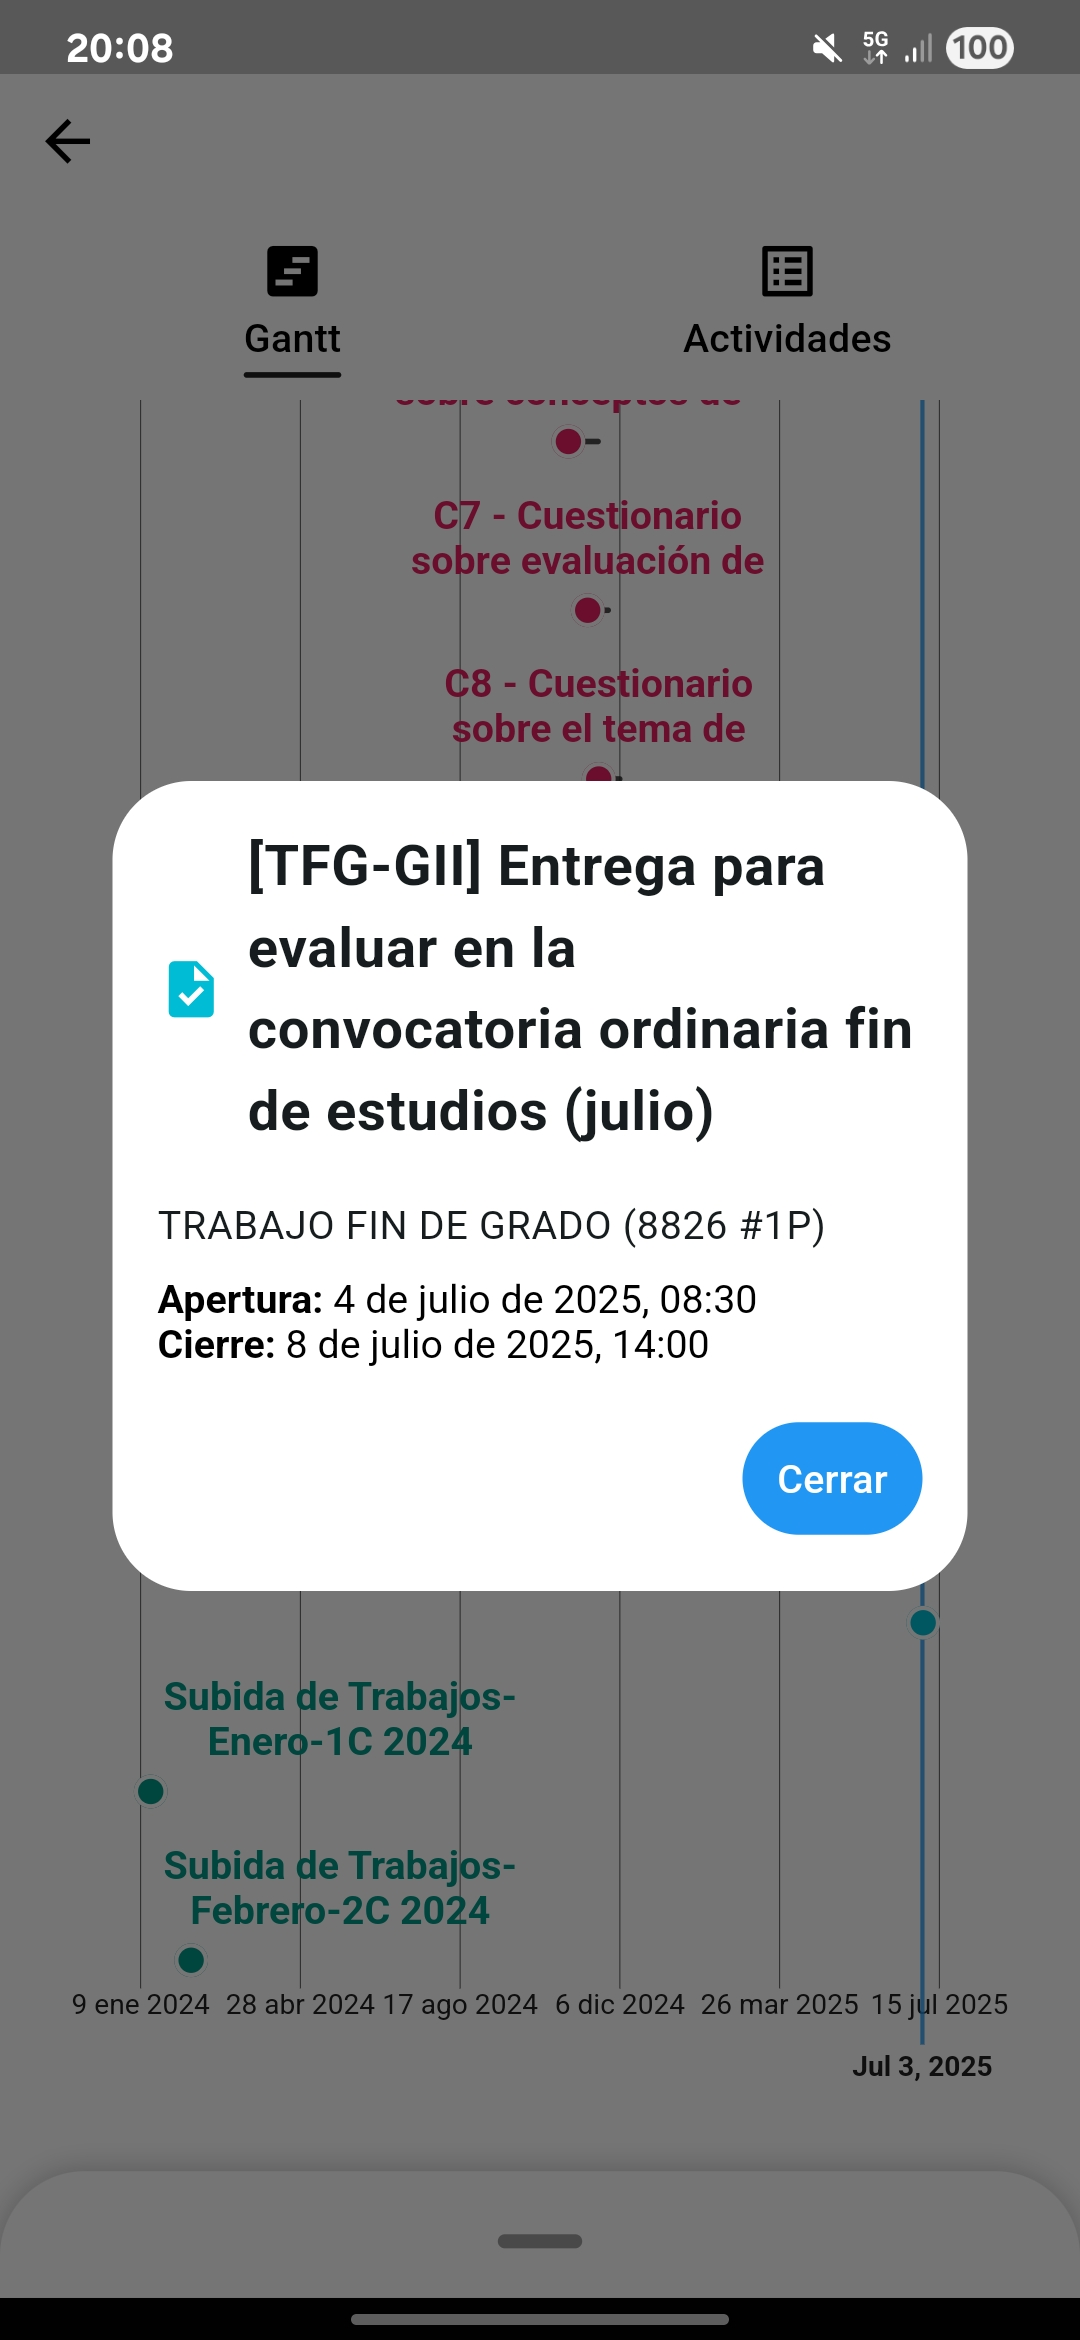
\includegraphics[width=0.5\linewidth]{img/gantt_actividad.jpg}}
     {\caption{Diálogo de actividad en diagrama de Gantt}
     \label{fig:gantt_actividad}}
  \end{floatrow}
\end{figure}

Si se presiona cualquier punto de los que aparecen en el diagrama, se abrirá un pequeño diálogo con información de la actividad \ref{fig:gantt_actividad}.

En la parte inferior de la pantalla \ref{fig:diagrama_gantt}
se puede observar un pequeño panel que si es deslizado hacia arriba, mostrará dos filtros que permiten modificar la estética del diagrama.
\begin{figure}[H]
  \centering
  \begin{floatrow}
    \ffigbox
      {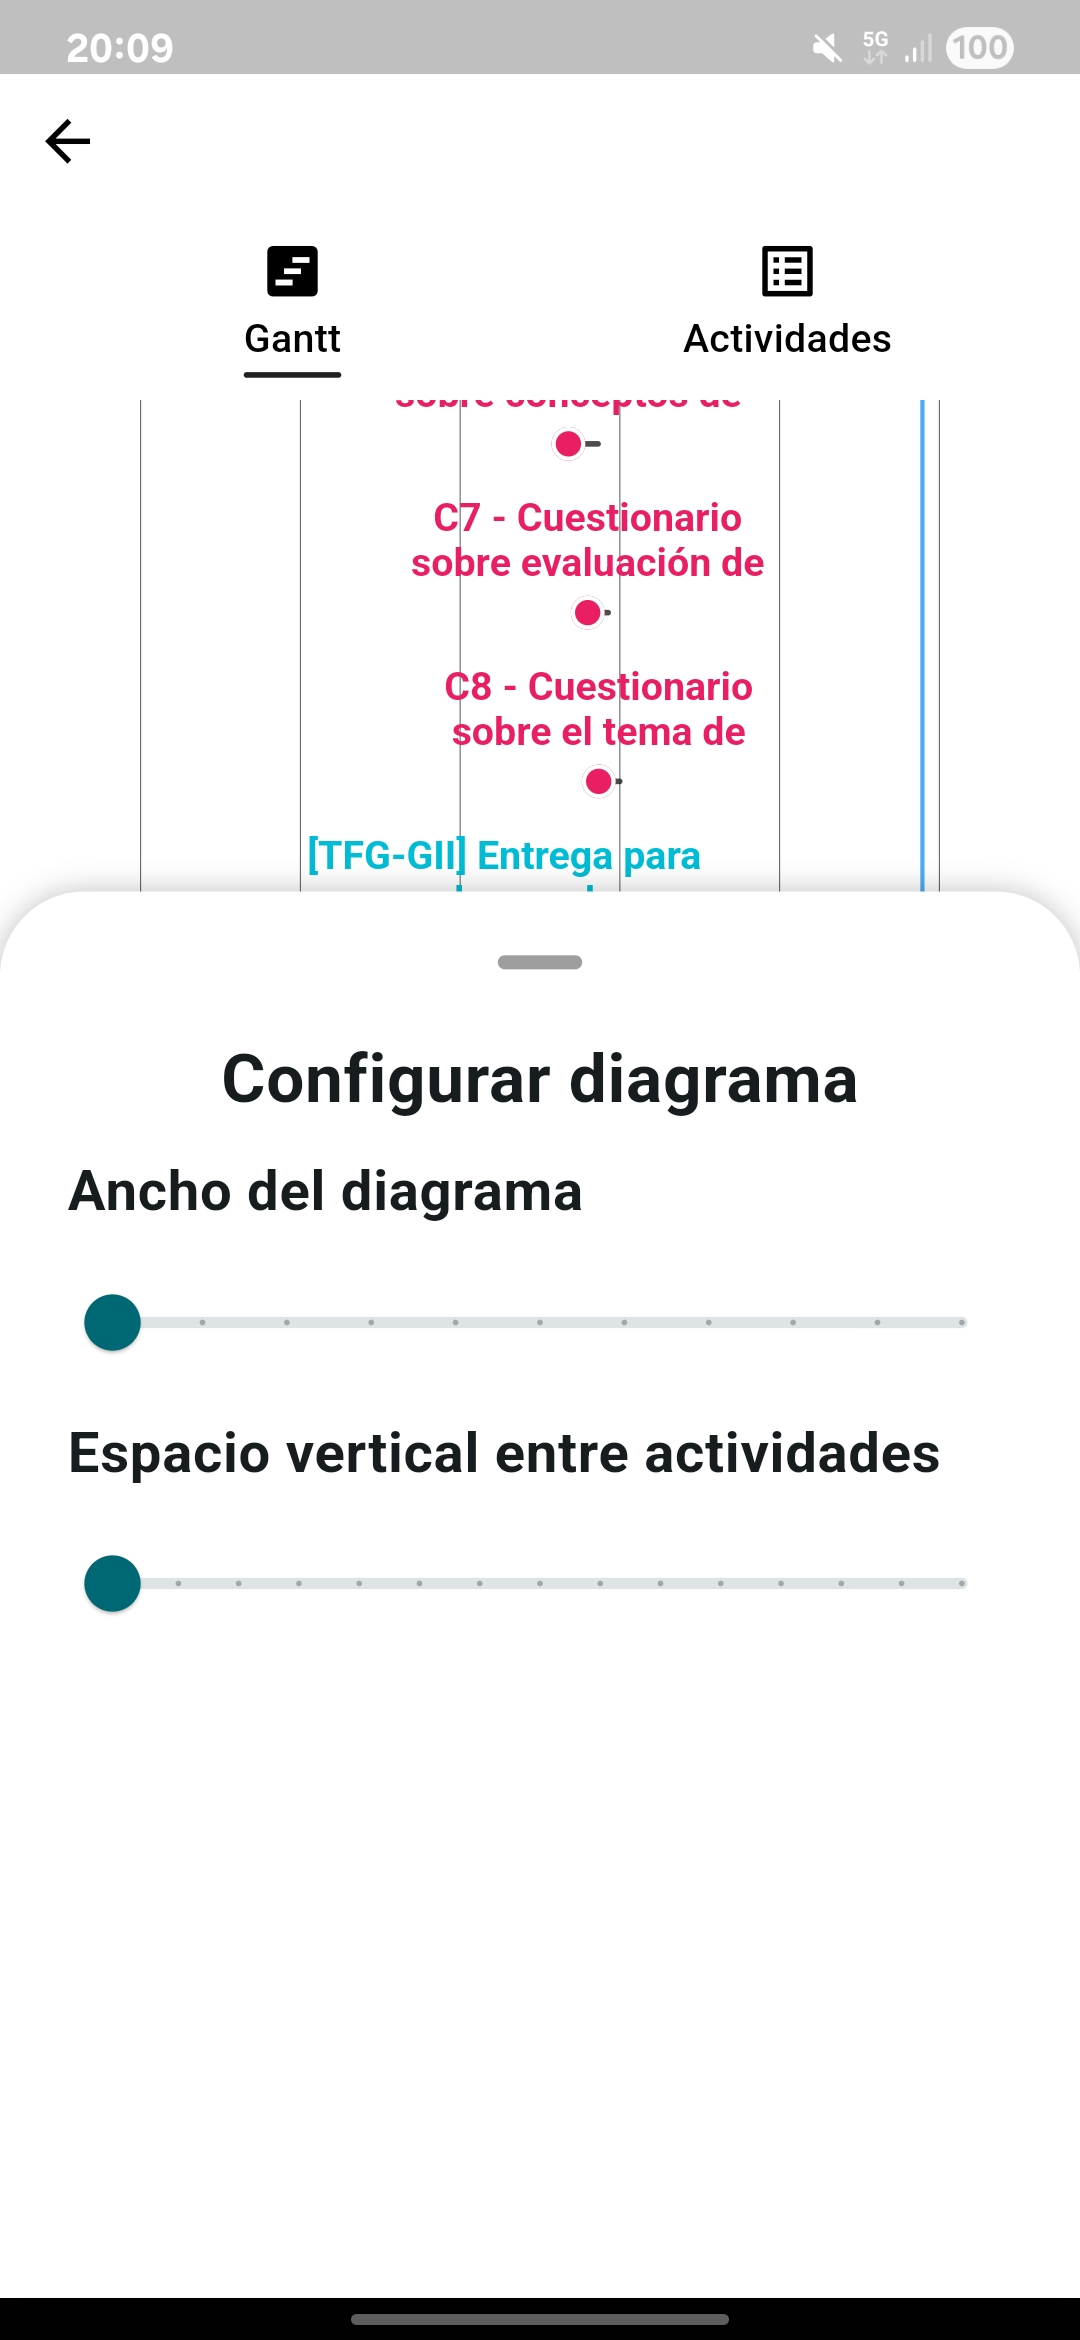
\includegraphics[width=0.5\linewidth]{img/filtros_diagrama.jpg}}
      {\caption{Filtros del diagrama de Gantt}
      \label{fig:filtros_diagrama}}
    \hfill
    \ffigbox
     {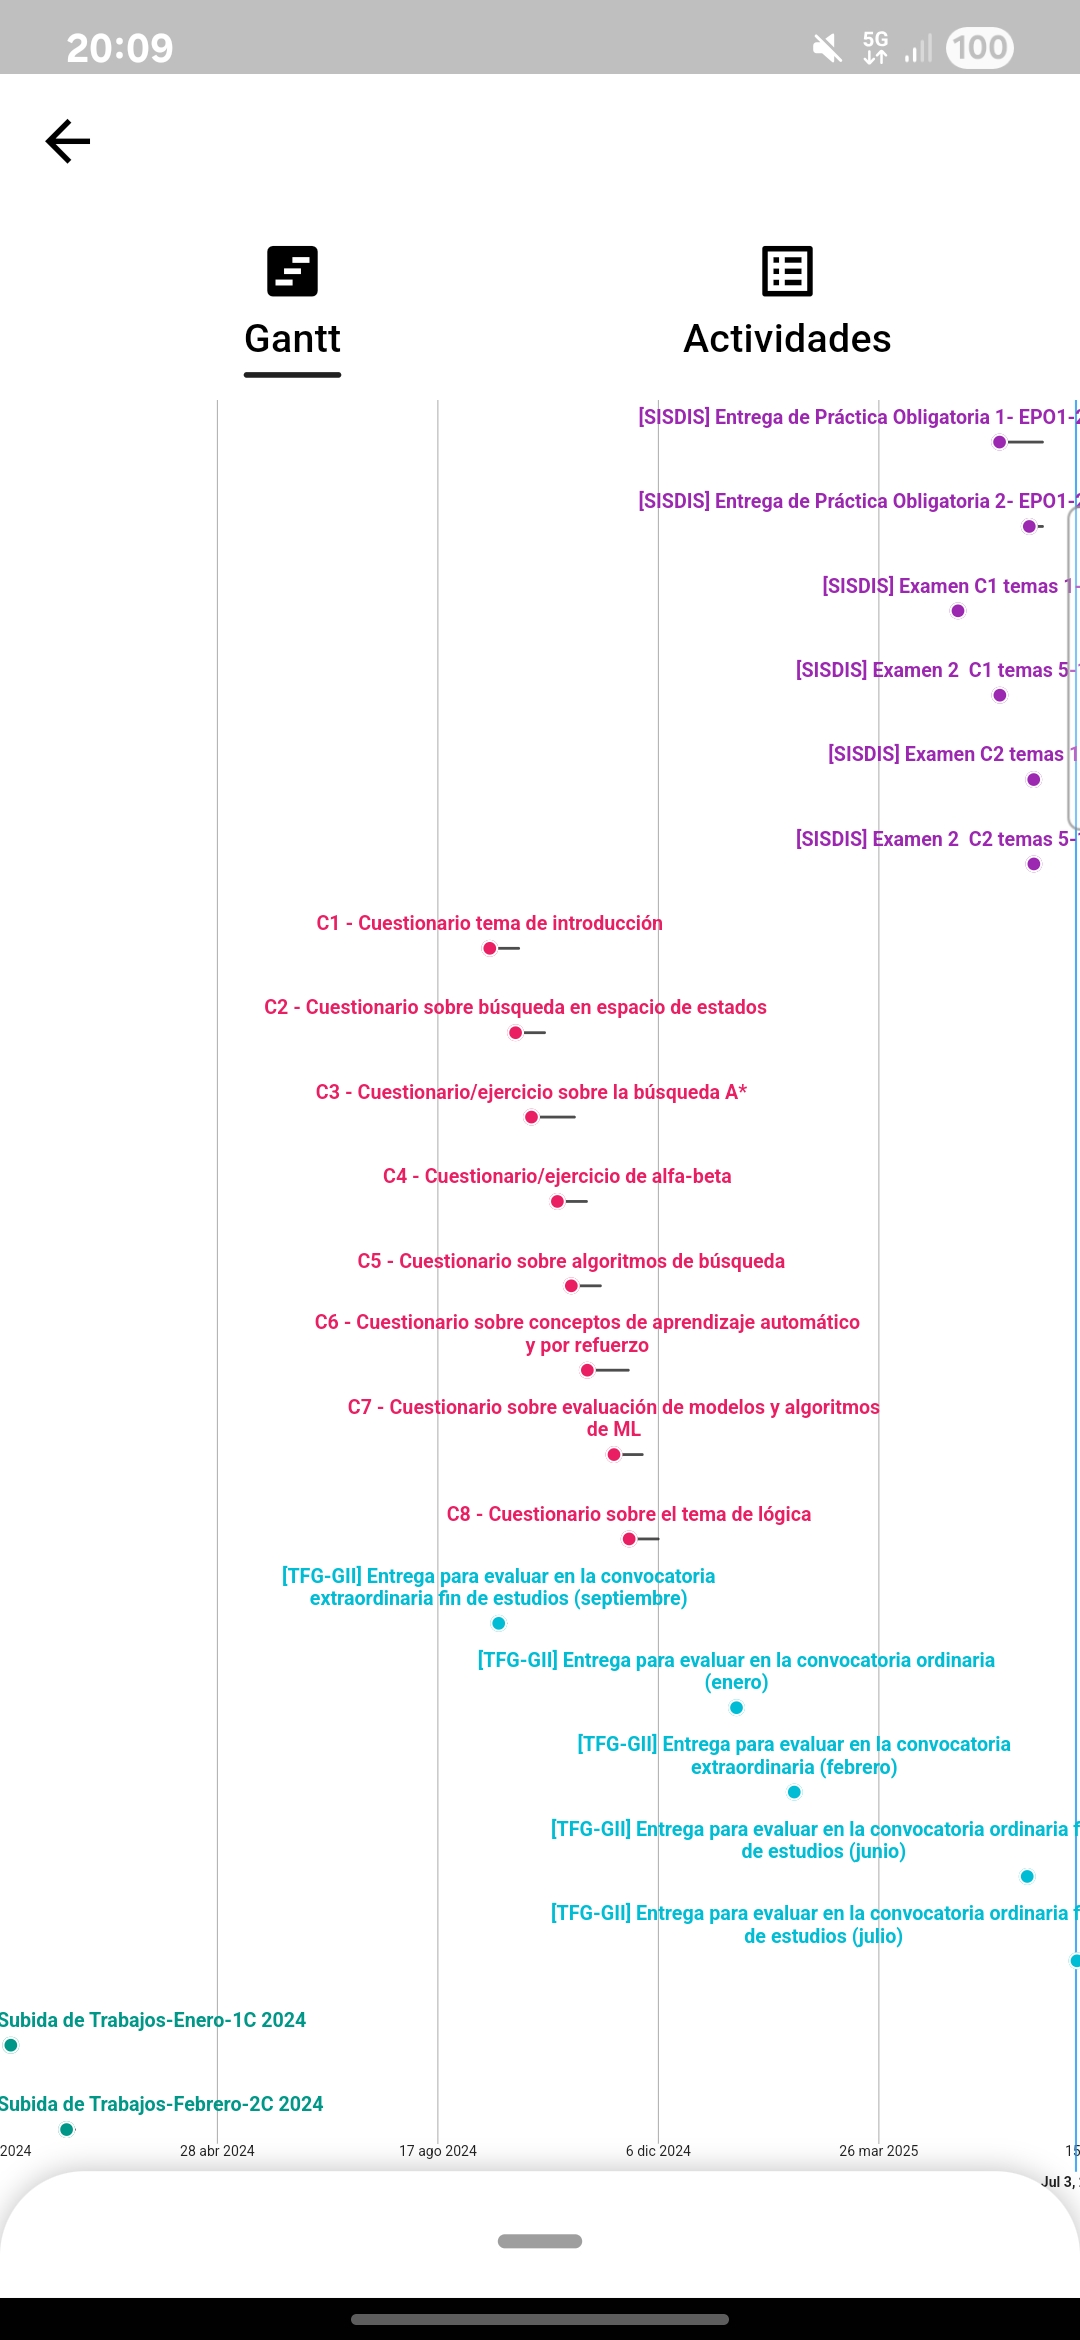
\includegraphics[width=0.5\linewidth]{img/diagrama_filtrado.jpg}}
     {\caption{Filtros estéticos aplicados sobre el diagrama}
     \label{fig:diagrama_filtrado}}
  \end{floatrow}
\end{figure}

Otra funcionalidad del diagrama, es que permite el desplazamiento en todas las direcciones, así como hacer \textit{zoom}, todo mediante gestos en la pantalla con los dedos.

Por otra parte, dentro de la pantalla del diagrama de Gantt, hay una sección de actividades \ref{fig:tareas_gantt}, en la cual aparecen todas las actividades que se encuentren dibujadas en el diagrama de Gantt.
\begin{figure}[H]
    \centering
    {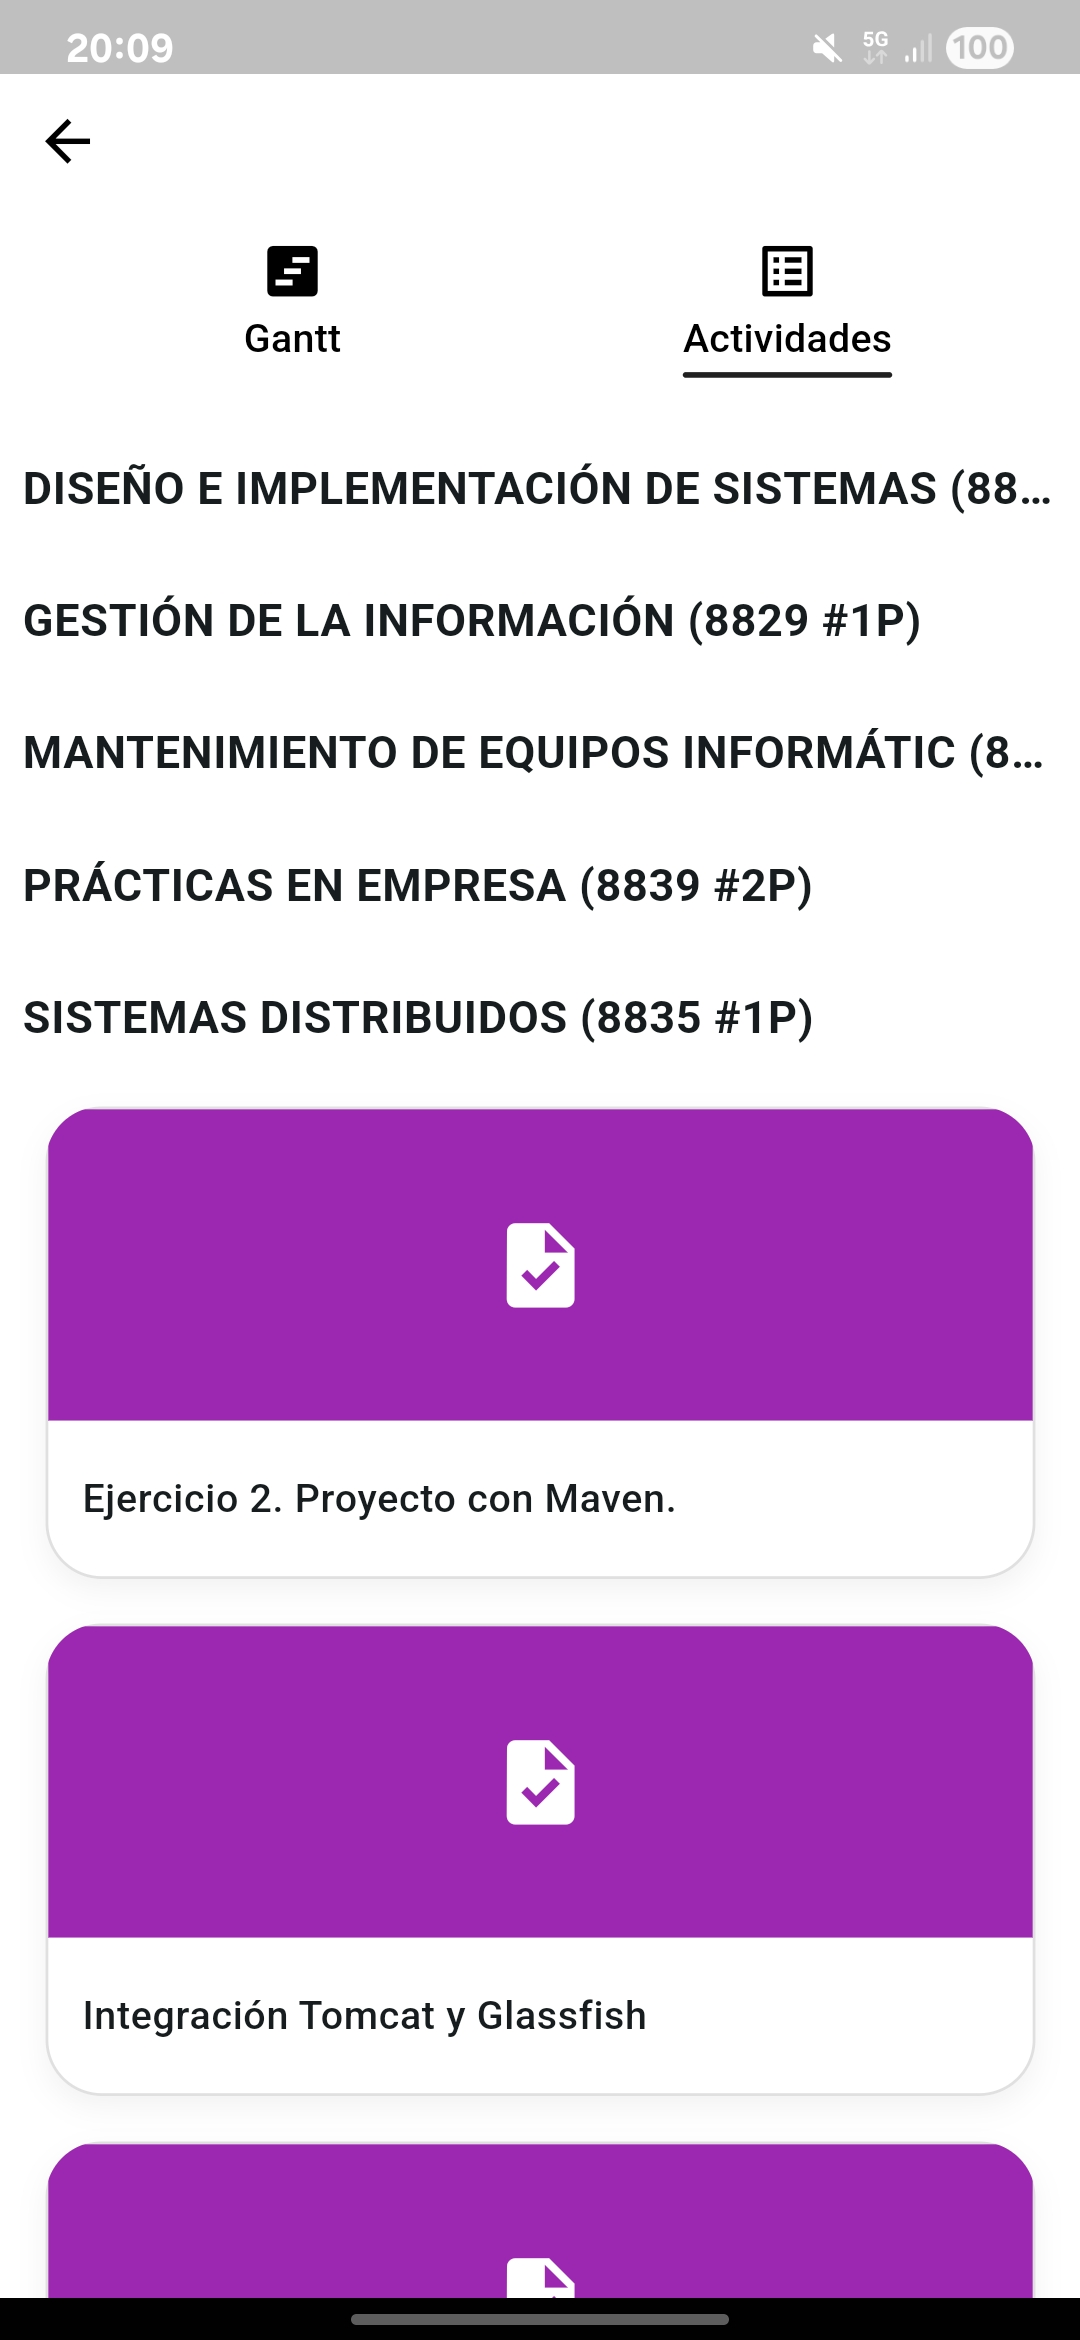
\includegraphics[width=0.25\linewidth]{img/tareas_gantt.jpg}}
    {\caption{Sección de actividades del diagrama de Gantt}
    \label{fig:tareas_gantt}}
\end{figure}

Al presionar una de las tarjetas que aparecen, se despliega una nueva ventana \ref{fig:tarea_gantt} con toda la información que se recoge de Moodle y que pueda llegar a ser útil para el usuario.
\begin{figure}[H]
    \centering
    {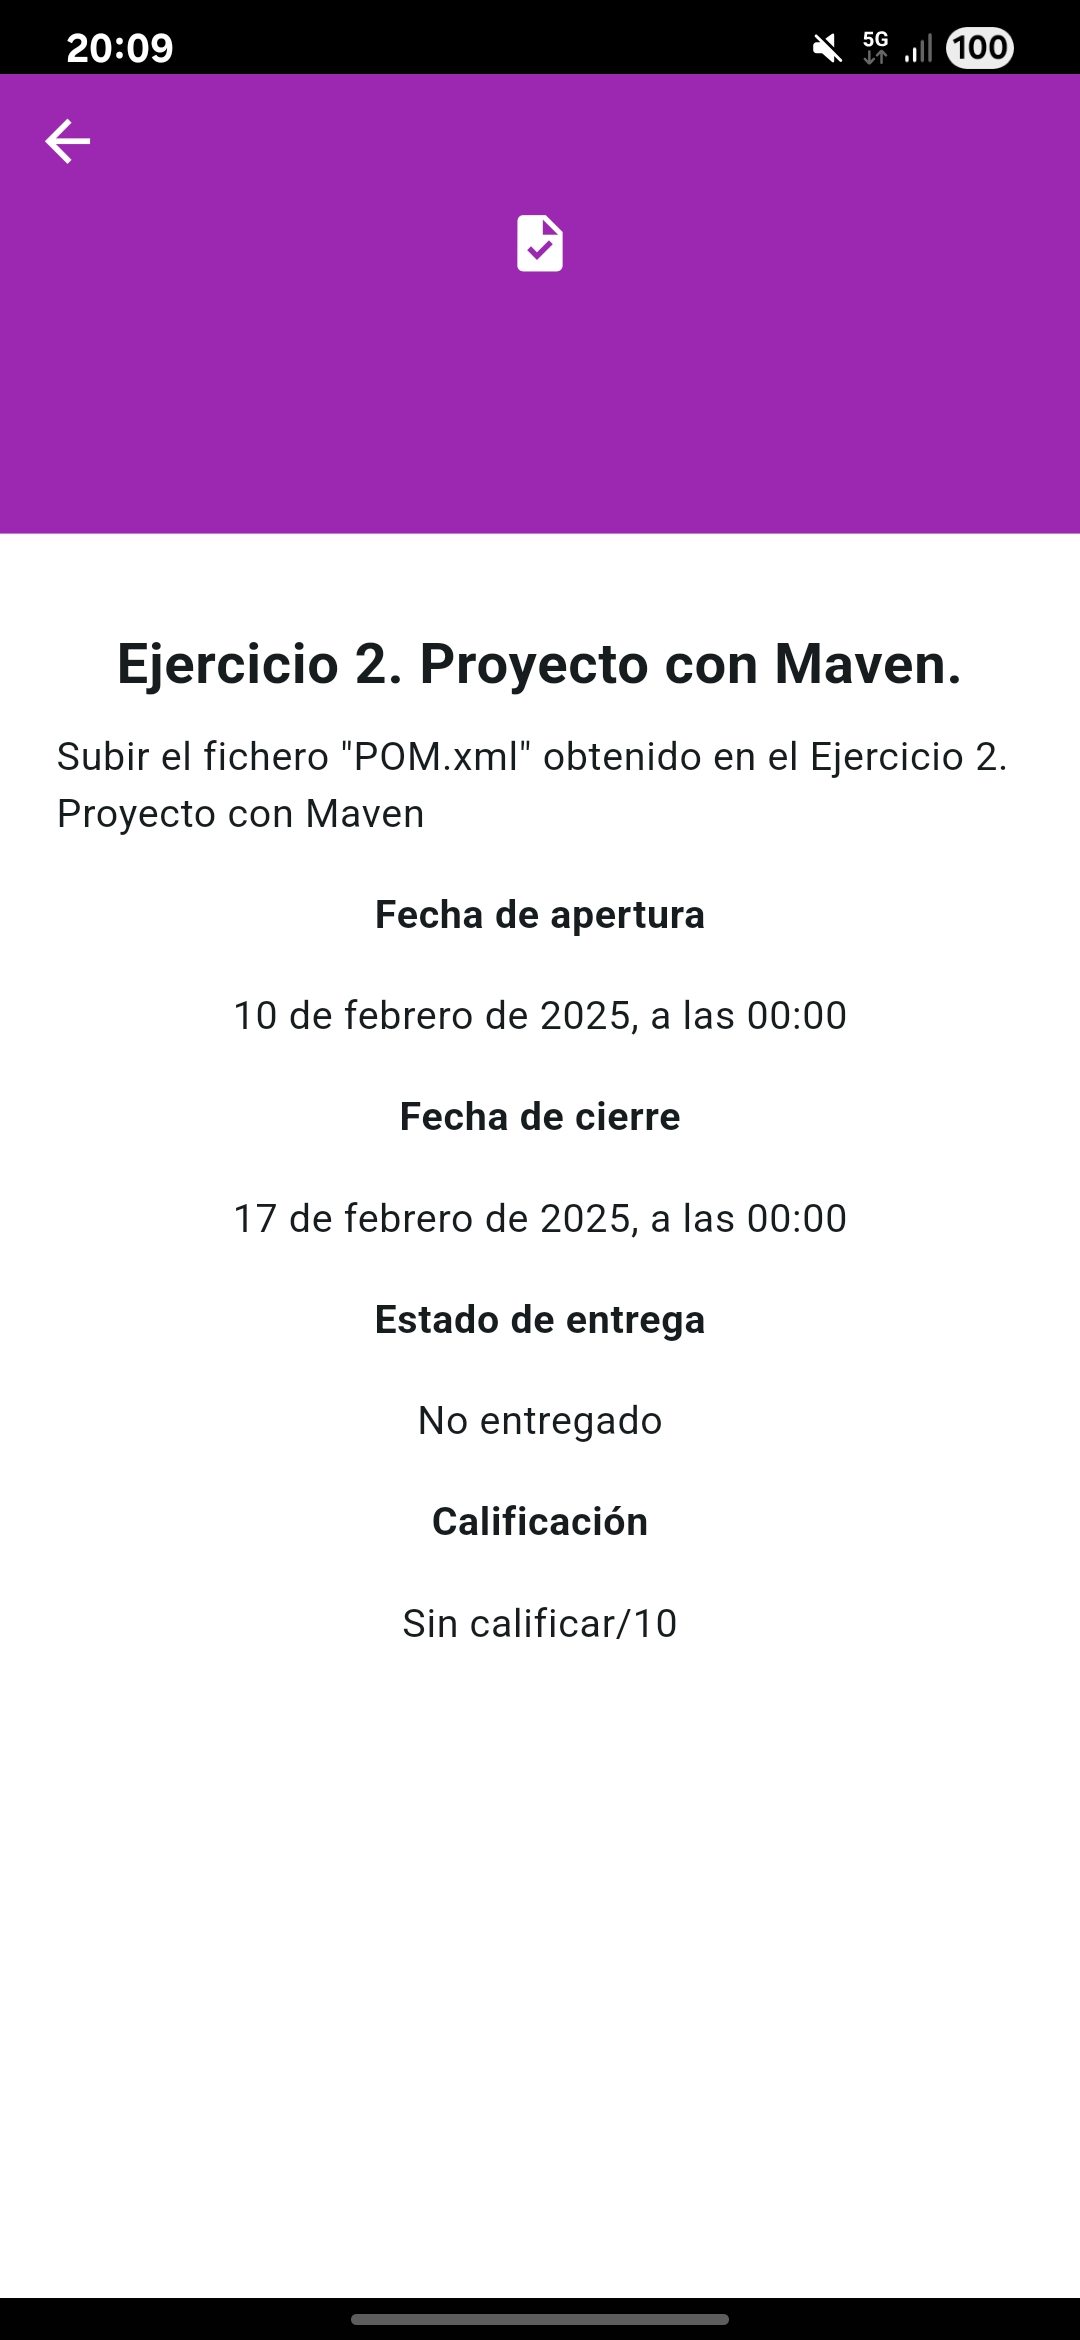
\includegraphics[width=0.25\linewidth]{img/tarea_gantt.jpg}}
     {\caption{Ventana con información de la actividad}
     \label{fig:tarea_gantt}}
\end{figure}

\subsubsection{Tareas Personales}
La última funcionalidad a explicar, son la tareas personales. Esta función tiene acceso desde la pantalla principal \ref{fig:pantalla_principal} y permite al usuario crear sus propias tareas personales con información personalizada.

Dentro de esta pantalla existen dos secciones: \textit{Pendientes} y \textit{Completadas}. Como su propio nombre indica, hacen referencia al estado de finalización de la tarea. A su vez, dentro de cada sección hay distintas subsecciones:
\begin{itemize}
    \item \textbf{Pendientes:} Hoy, Mañana, Esta Semana y Todos
    \item \textbf{Completadas:} Hoy, Últimos 7d, Este mes y Todos
\end{itemize}
\begin{figure}[H]
  \centering
  \begin{floatrow}
    \ffigbox
      {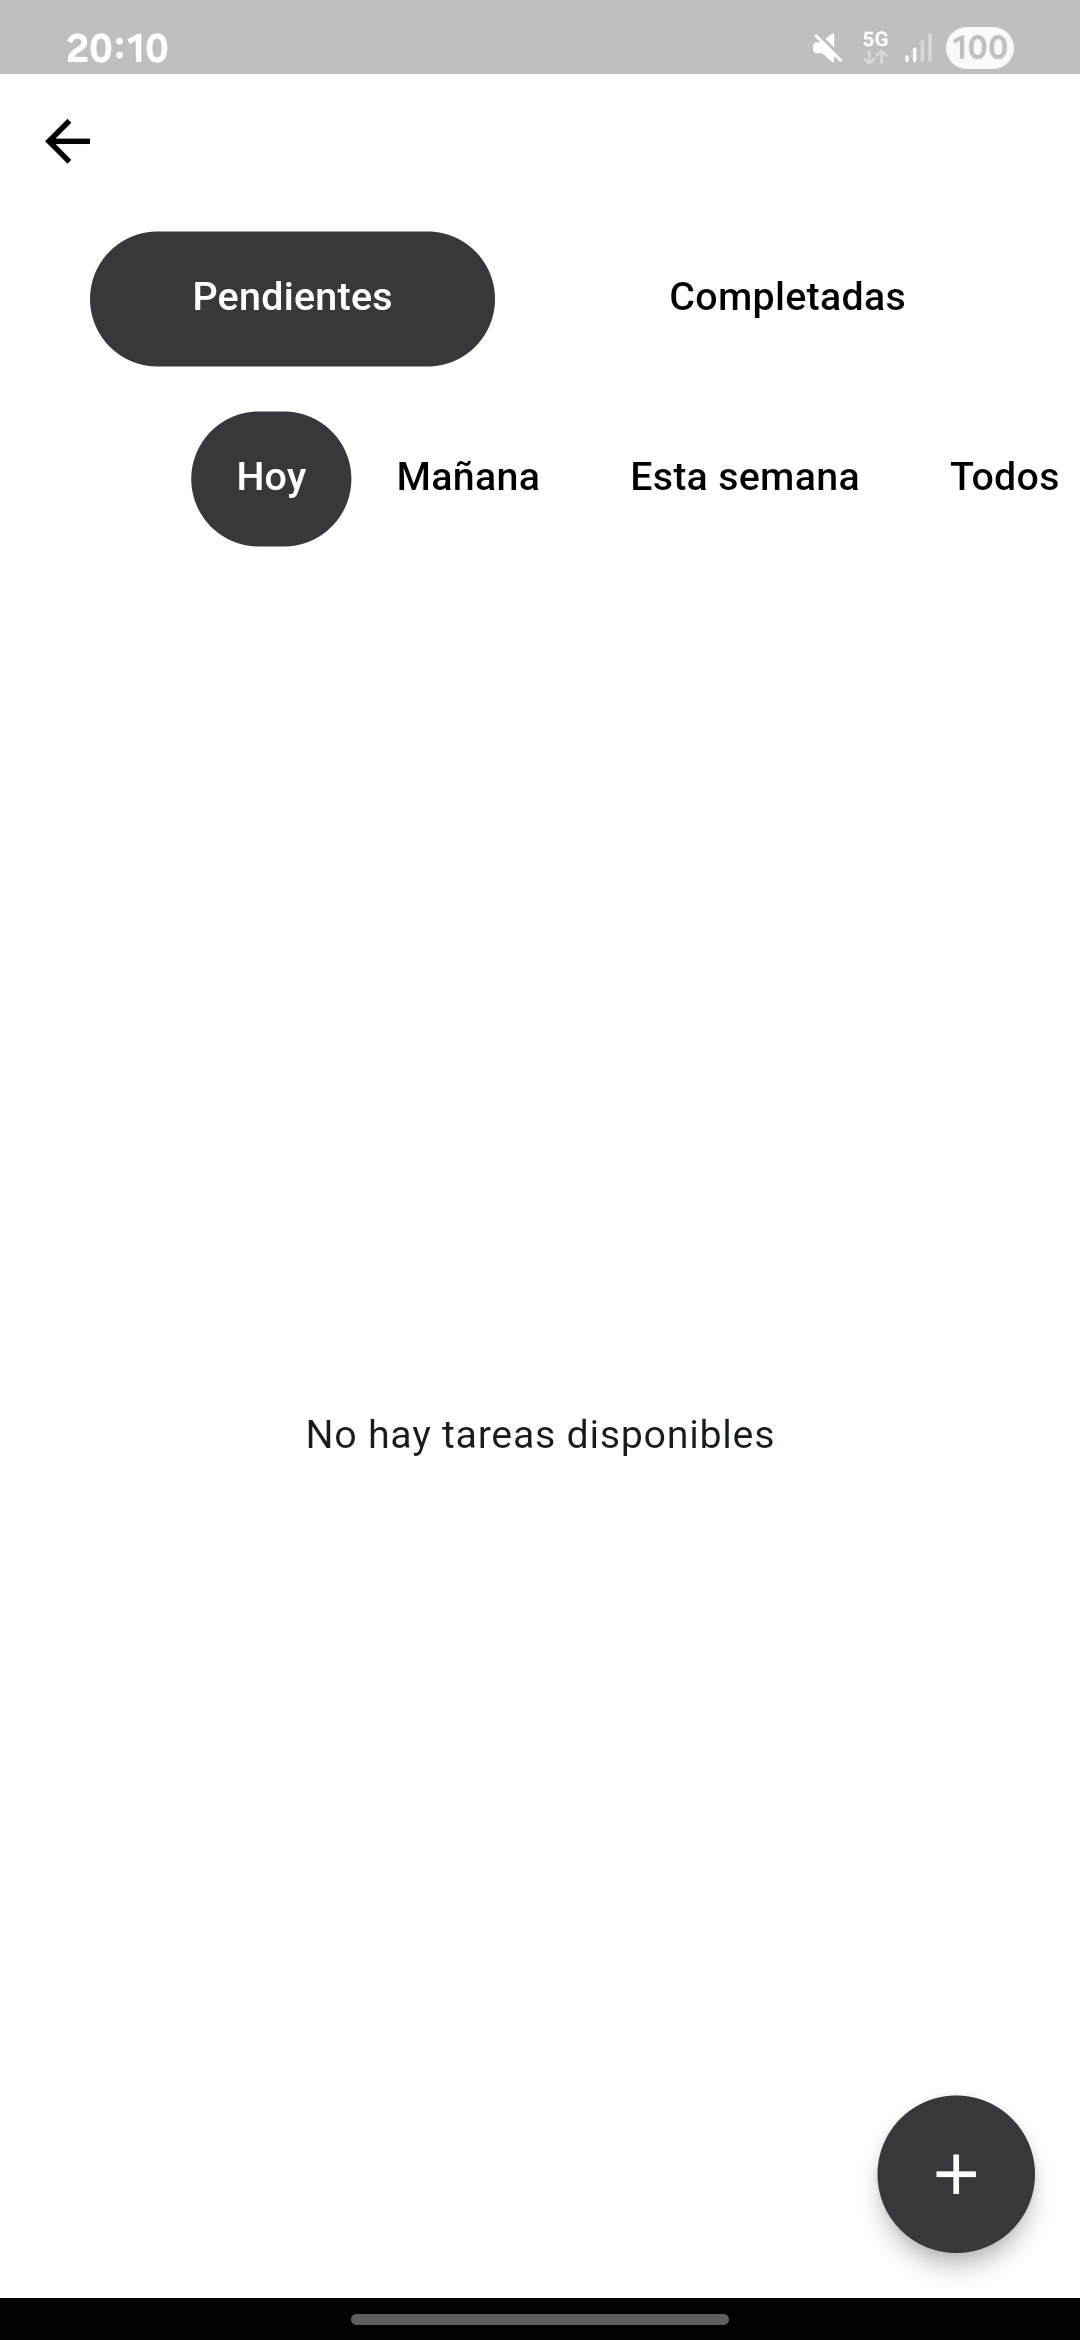
\includegraphics[width=0.5\linewidth]{img/tareas_personales_pendientes.jpg}}
      {\caption{Sección de tareas pendientes}
      \label{fig:tareas_personales_pendientes}}
    \hfill
    \ffigbox
     {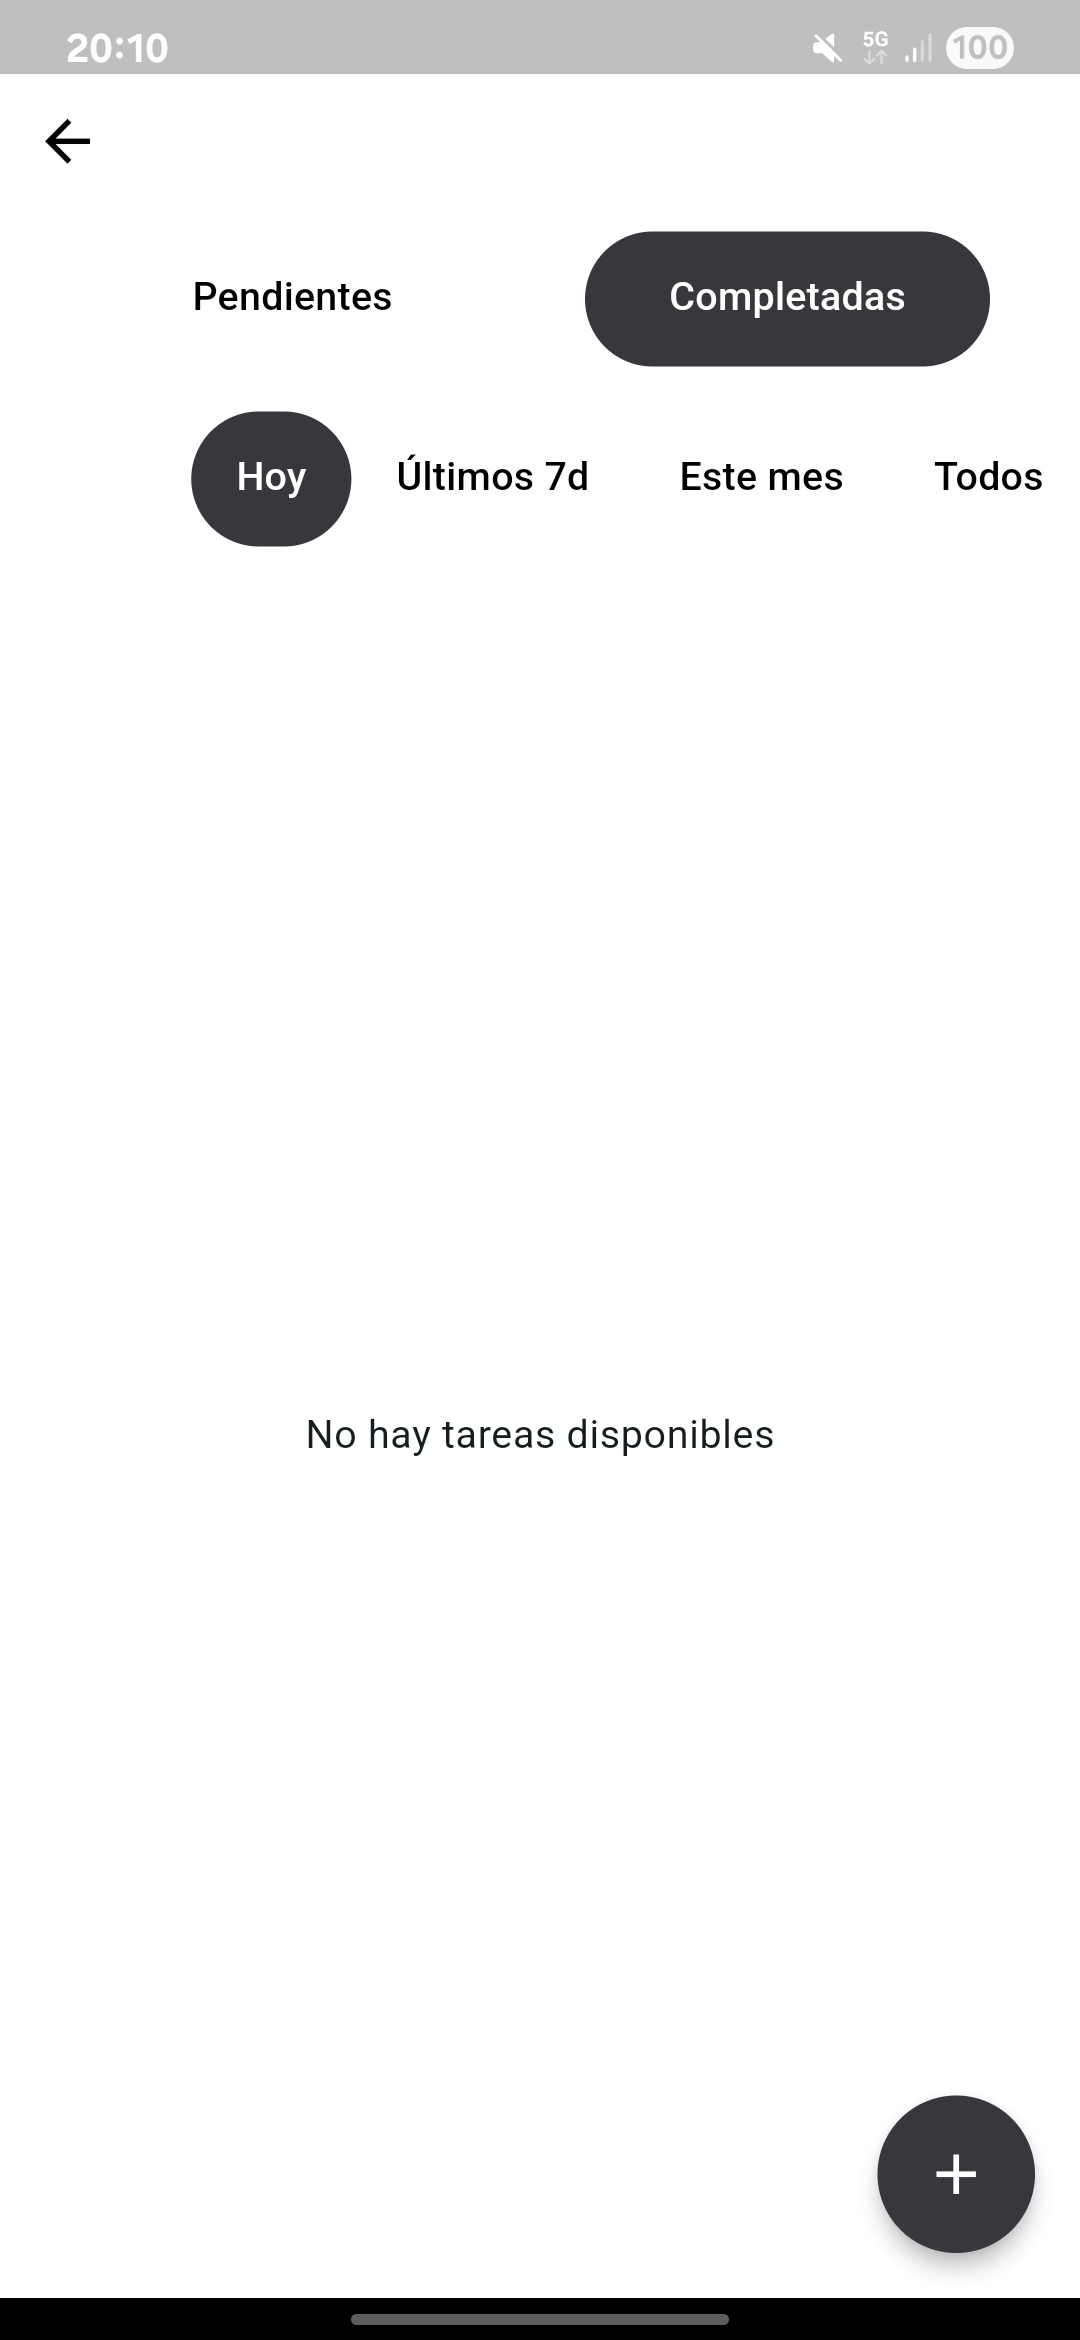
\includegraphics[width=0.5\linewidth]{img/tareas_personales_completadas.jpg}}
     {\caption{Sección de tareas completadas}
     \label{fig:tareas_personales_completadas}}
  \end{floatrow}
\end{figure}

En la parte inferior derecha de la pantalla \ref{fig:tareas_personales_pendientes} se encuentra un botón que al ser pulsado abre una ventana con un formulario de \textit{Creación de tareas}. El cual consta de unos campos obligatorios y otros opcionales. Una vez rellenados los campos y guardada la tarea, esta se añade directamente a la sección de tareas pendientes.
\begin{figure}[H]
  \centering
  \begin{floatrow}
    \ffigbox
      {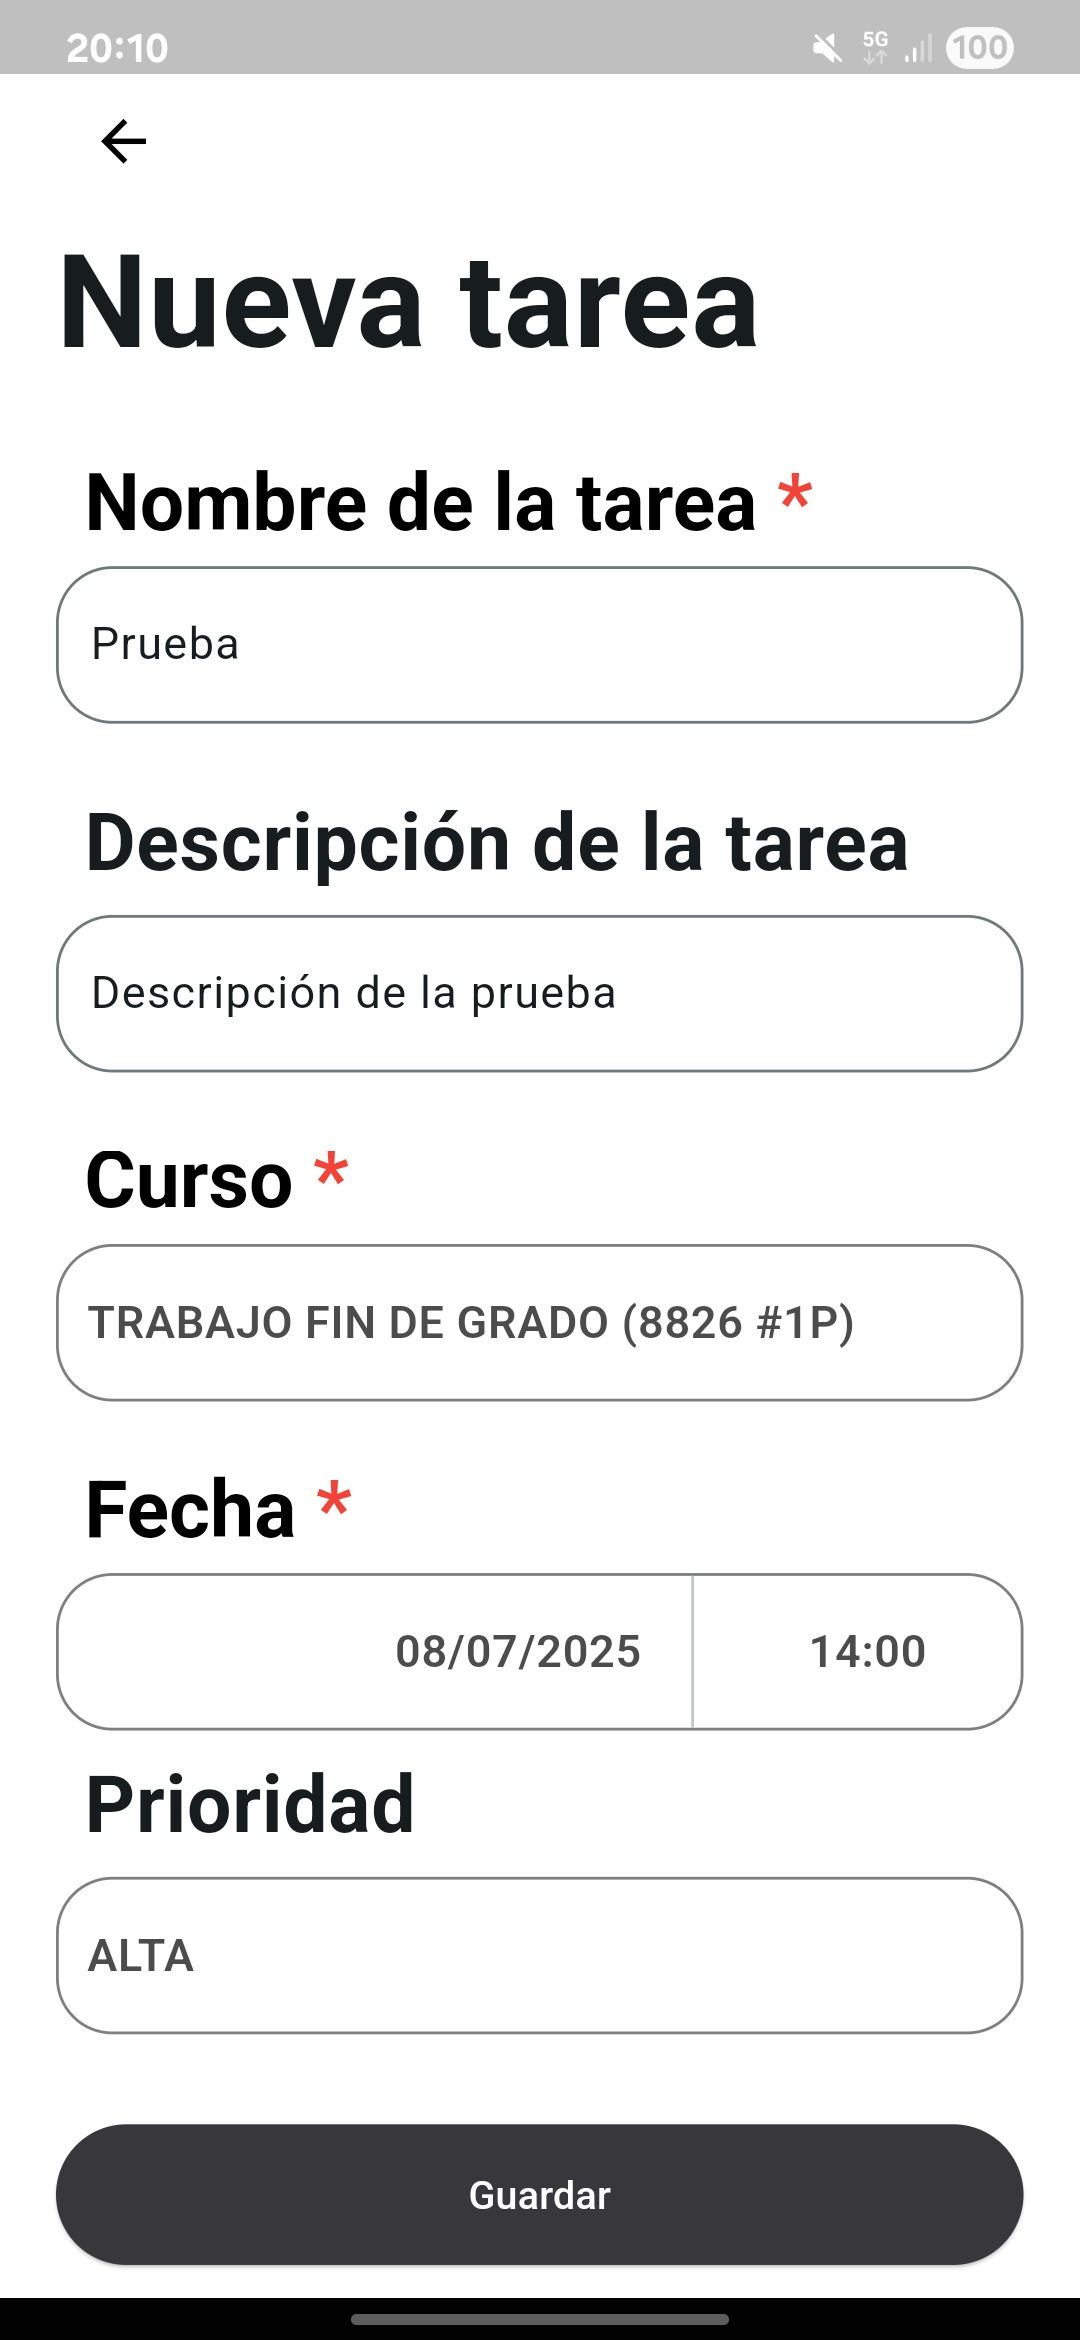
\includegraphics[width=0.5\linewidth]{img/formulario_rellenado.jpg}}
      {\caption{Formulario de creación de tareas personales}
      \label{fig:formulario_rellenado}}
    \hfill
    \ffigbox
     {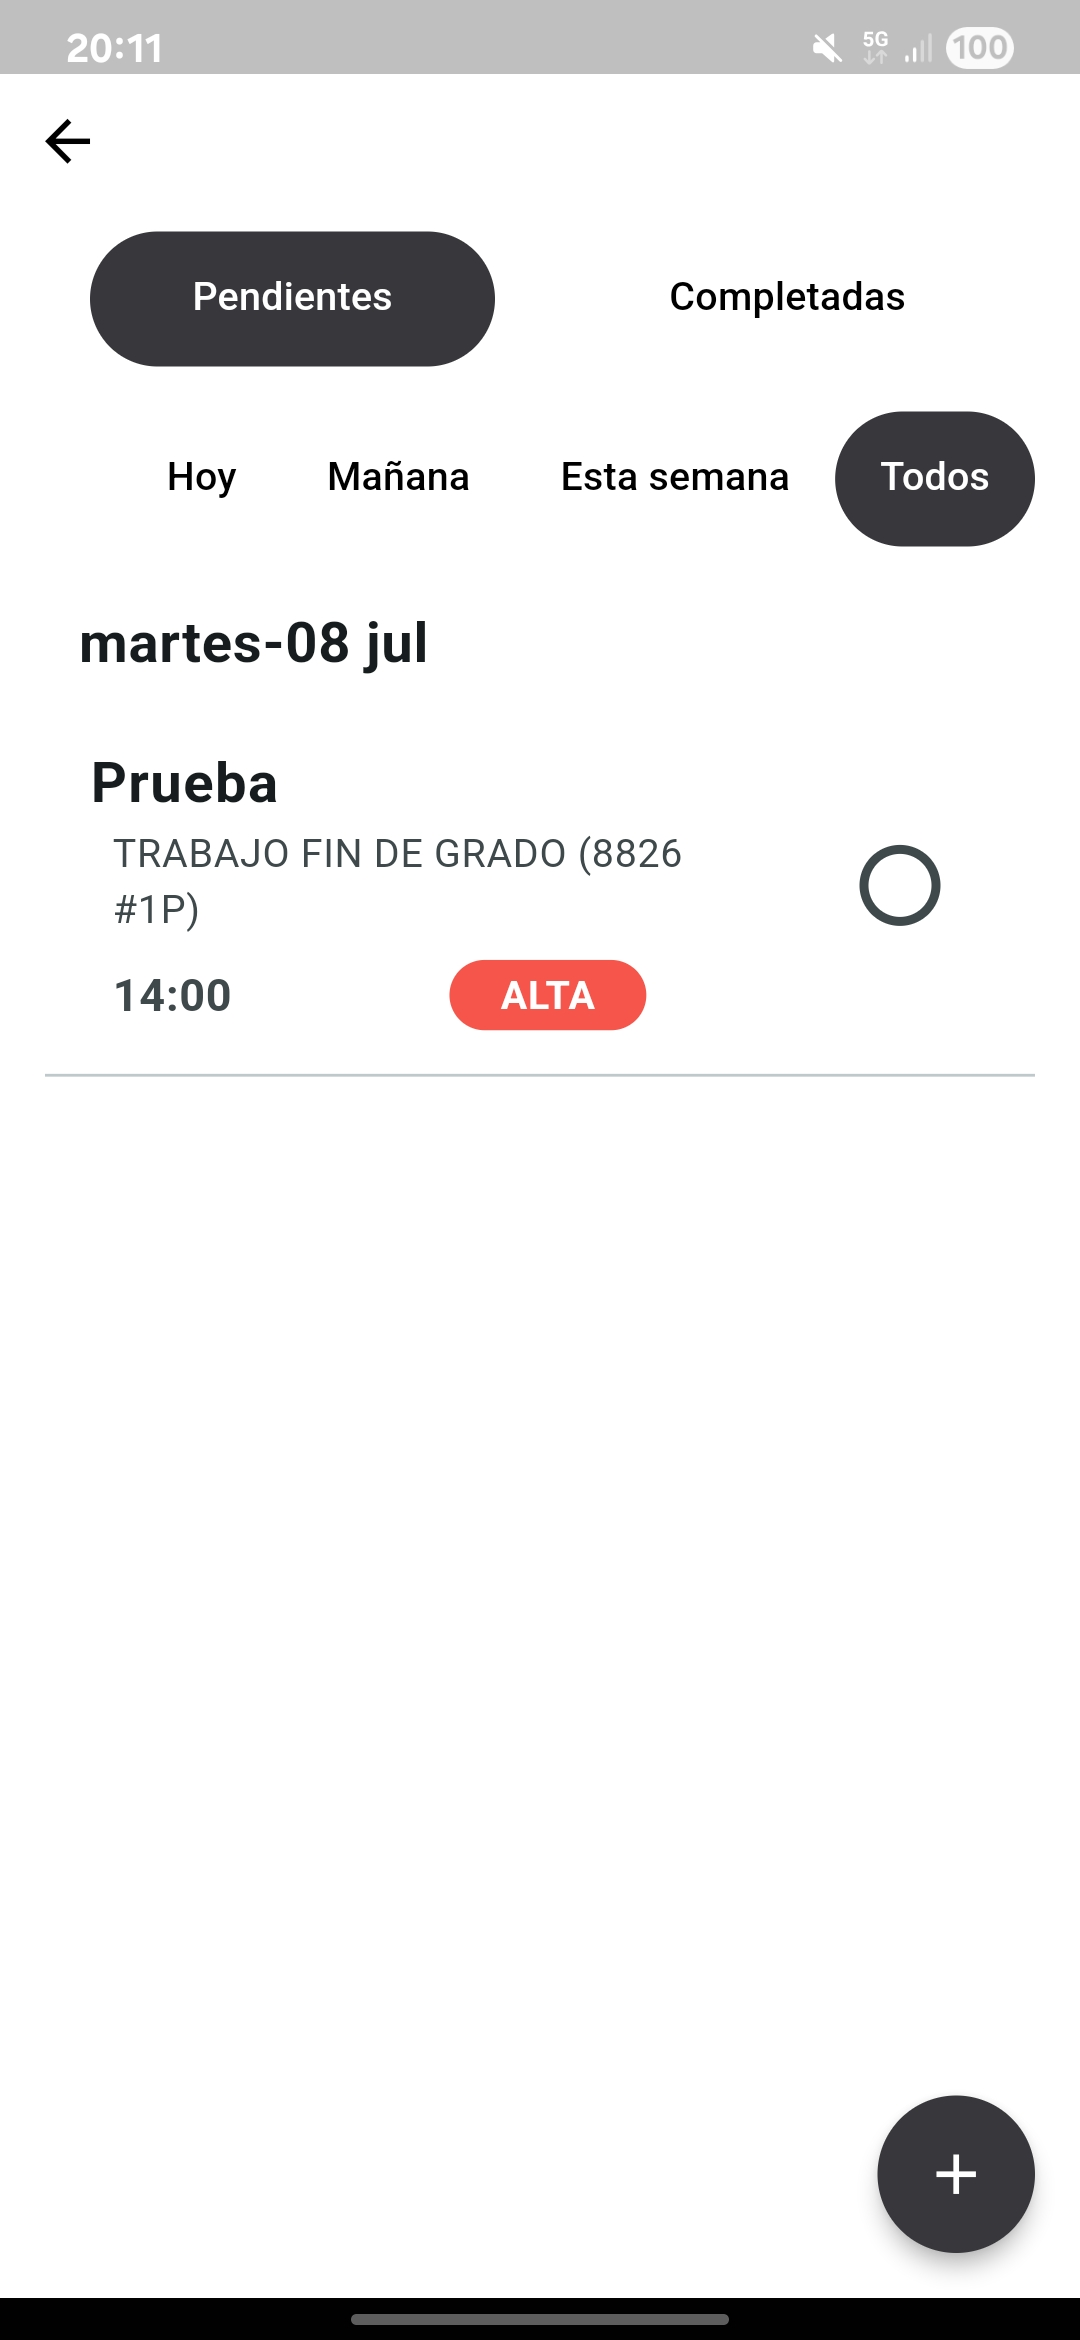
\includegraphics[width=0.5\linewidth]{img/tarea_personal.jpg}}
     {\caption{Tarea personal en sección de \textit{Pendientes}}
     \label{fig:tarea_personal}}
  \end{floatrow}
\end{figure}

Al presionar la tarea personal creada, aparecerá un panel con toda la información de dicha tarea \ref{fig:visualizacion_tarea_personal}.
\begin{figure}[H]
    \centering
    {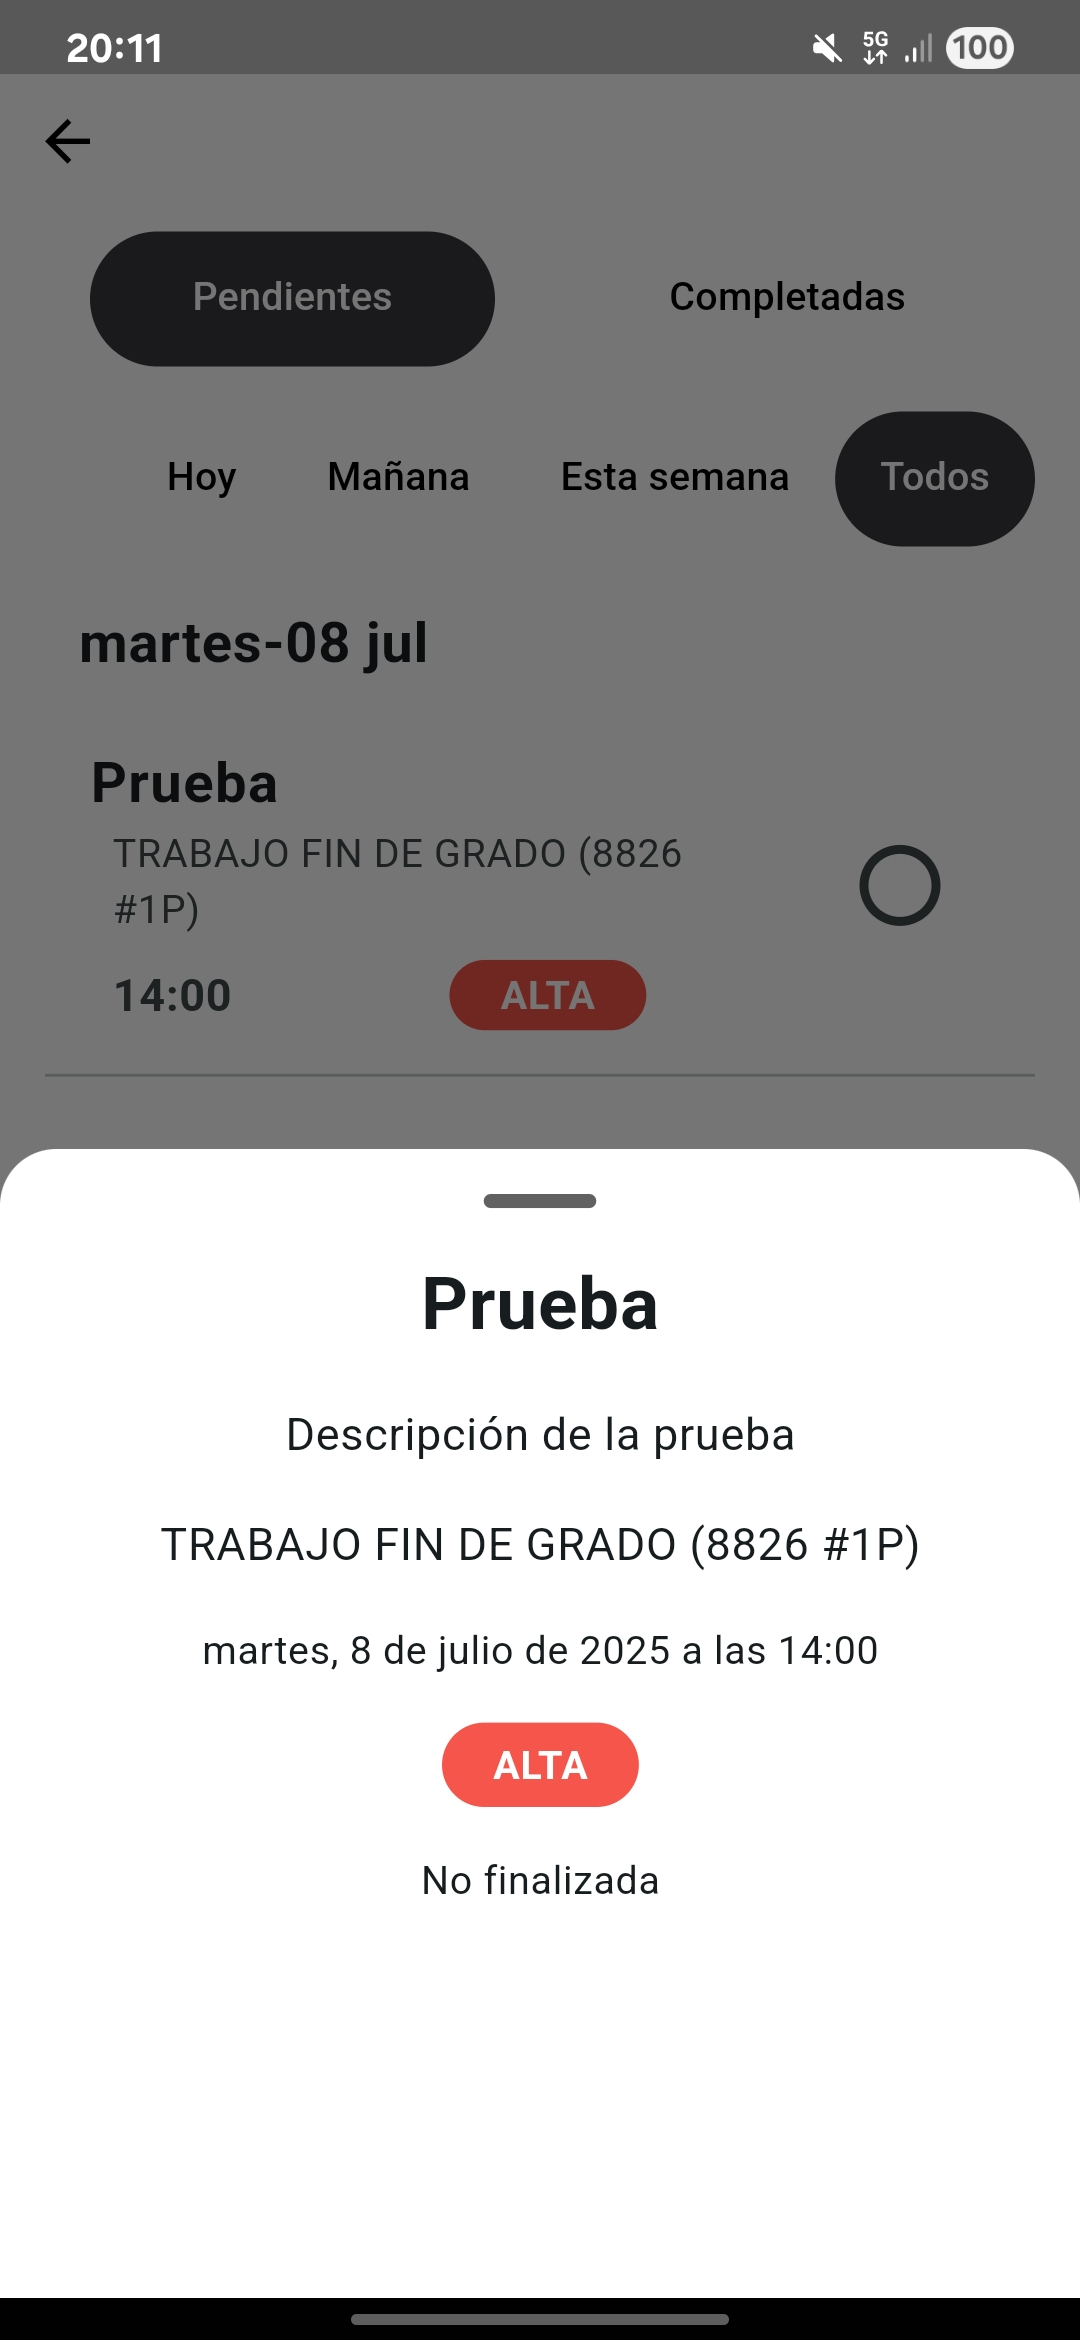
\includegraphics[width=0.25\linewidth]{img/visualizacion_tarea_personal.jpg}}
     {\caption{Panel con información de la tarea personal}
     \label{fig:visualizacion_tarea_personal}}
\end{figure}

El circulo que aparece en la tarea de la pantalla \ref{fig:tarea_personal}, al ser presionado marca la tarea como \textit{Completada} y se moverá directamente a la sección correspondiente.

Por último, si se desliza la tarea de derecha a izquierda, se descubrirá la opción de borrado de la tarea \ref{fig:eliminar_tarea}.
\begin{figure}[H]
    \centering
    {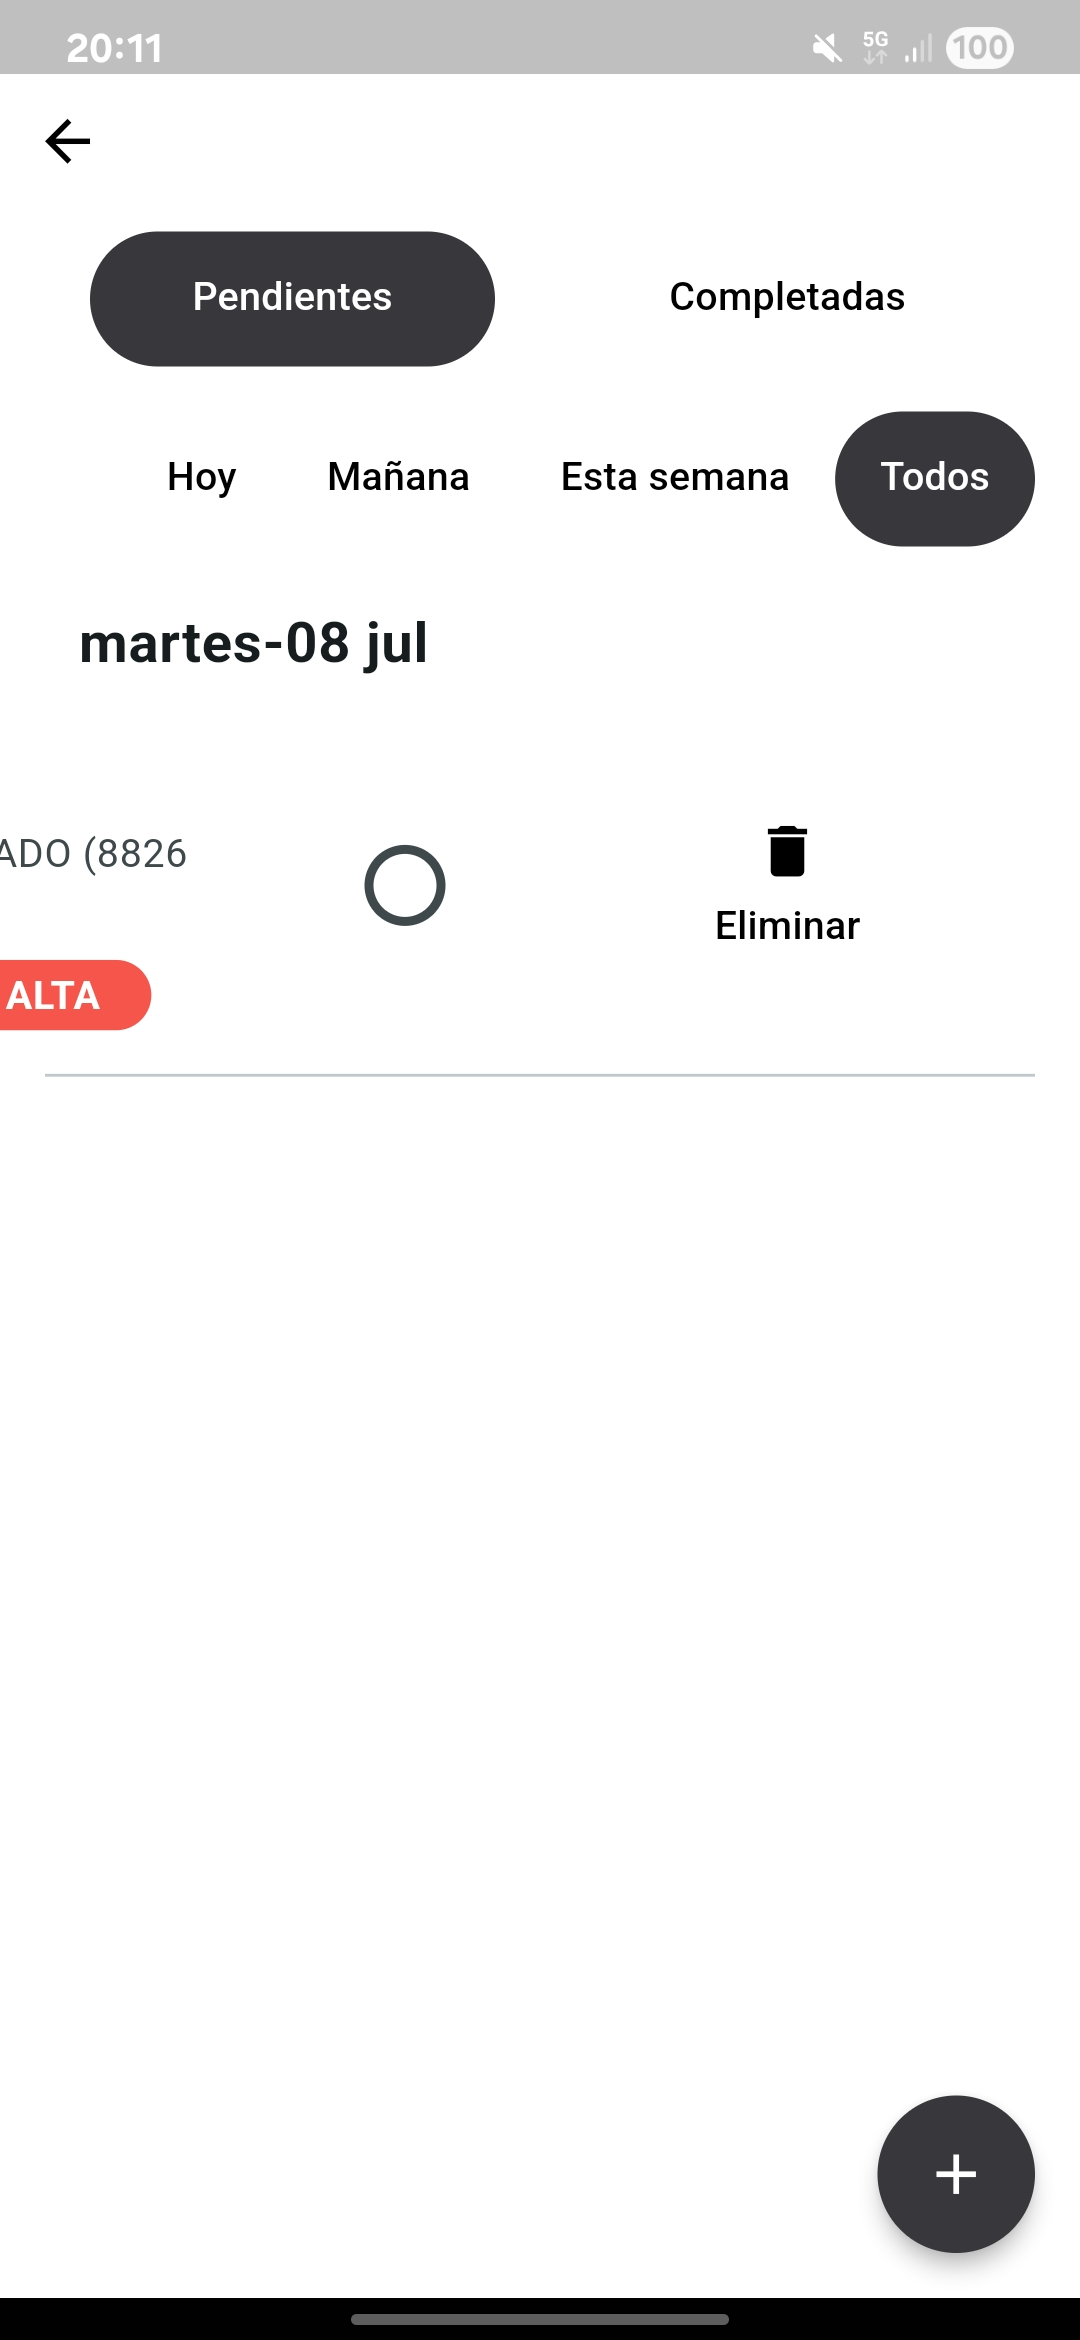
\includegraphics[width=0.25\linewidth]{img/eliminar_tarea.jpg}}
     {\caption{Opción de borrado de la tarea personal}
     \label{fig:eliminar_tarea}}
\end{figure}